\documentclass{beamer}
\usepackage[italian]{babel}
\usetheme{Berkeley}
\usepackage{graphicx}
\usepackage{booktabs}
% Taken from Lena Herrmann at 
% http://lenaherrmann.net/2010/05/20/javascript-syntax-highlighting-in-the-latex-listings-package
\usepackage{listings,lstautogobble,longtable}
\usepackage{color} %use color
\definecolor{mygreen}{rgb}{0,0.6,0}
\definecolor{mygray}{rgb}{0.5,0.5,0.5}
\definecolor{mymauve}{rgb}{0.58,0,0.82}
% Copyright 2017 Sergei Tikhomirov, MIT License
% https://github.com/s-tikhomirov/solidity-latex-highlighting/

\usepackage{listings, xcolor}

\definecolor{verylightgray}{rgb}{.97,.97,.97}

\lstdefinelanguage{Solidity}{
	keywords=[1]{anonymous, assembly, assert, balance, break, call, callcode, case, catch, class, constant, continue, constructor, contract, debugger, default, delegatecall, delete, do, else, emit, event, experimental, export, external, false, finally, for, function, gas, if, implements, import, in, indexed, instanceof, interface, internal, is, length, library, log0, log1, log2, log3, log4, memory, modifier, new, payable, pragma, private, protected, public, pure, push, require, return, returns, revert, selfdestruct, send, solidity, storage, struct, suicide, super, switch, then, this, throw, transfer, true, try, typeof, using, value, view, while, with, addmod, ecrecover, keccak256, mulmod, ripemd160, sha256, sha3}, % generic keywords including crypto operations
	keywordstyle=[1]\color{blue}\bfseries,
	keywords=[2]{address, bool, byte, bytes, bytes1, bytes2, bytes3, bytes4, bytes5, bytes6, bytes7, bytes8, bytes9, bytes10, bytes11, bytes12, bytes13, bytes14, bytes15, bytes16, bytes17, bytes18, bytes19, bytes20, bytes21, bytes22, bytes23, bytes24, bytes25, bytes26, bytes27, bytes28, bytes29, bytes30, bytes31, bytes32, enum, int, int8, int16, int24, int32, int40, int48, int56, int64, int72, int80, int88, int96, int104, int112, int120, int128, int136, int144, int152, int160, int168, int176, int184, int192, int200, int208, int216, int224, int232, int240, int248, int256, mapping, string, uint, uint8, uint16, uint24, uint32, uint40, uint48, uint56, uint64, uint72, uint80, uint88, uint96, uint104, uint112, uint120, uint128, uint136, uint144, uint152, uint160, uint168, uint176, uint184, uint192, uint200, uint208, uint216, uint224, uint232, uint240, uint248, uint256, var, void, ether, finney, szabo, wei, days, hours, minutes, seconds, weeks, years},	% types; money and time units
	keywordstyle=[2]\color{teal}\bfseries,
	keywords=[3]{block, blockhash, coinbase, difficulty, gaslimit, number, timestamp, msg, data, gas, sender, sig, value, now, tx, gasprice, origin},	% environment variables
	keywordstyle=[3]\color{violet}\bfseries,
	identifierstyle=\color{black},
	sensitive=false,
	comment=[l]{//},
	morecomment=[s]{/*}{*/},
	commentstyle=\color{gray}\ttfamily,
	stringstyle=\color{red}\ttfamily,
	morestring=[b]',
	morestring=[b]"
}

\lstset{
	language=Solidity,
	backgroundcolor=\color{verylightgray},
	extendedchars=true,
	basicstyle=\footnotesize\ttfamily,
	showstringspaces=false,
	showspaces=false,
	numbers=left,
	numberstyle=\footnotesize,
	numbersep=9pt,
	tabsize=2,
	breaklines=true,
	showtabs=false,
	captionpos=b
}

%Customize a bit the look
\lstset{ %
autogobble = true,
backgroundcolor=\color{white}, % choose the background color; you must add \usepackage{color} or \usepackage{xcolor}
basicstyle=\footnotesize, % the size of the fonts that are used for the code
breakatwhitespace=false, % sets if automatic breaks should only happen at whitespace
breaklines=true, % sets automatic line breaking
captionpos=b, % sets the caption-position to bottom
commentstyle=\color{mygreen}, % comment style
deletekeywords={...}, % if you want to delete keywords from the given language
escapeinside={<@}{@>}, % if you want to add LaTeX within your code
escapechar={|},
extendedchars=true, % lets you use non-ASCII characters; for 8-bits encodings only, does not work with UTF-8
frame=single, % adds a frame around the code
keywordstyle=\color{blue}, % keyword style
% language=Octave, % the language of the code
morekeywords={*,...}, % if you want to add more keywords to the set
numbers=left, % where to put the line-numbers; possible values are (none, left, right)
numbersep=0pt, % how far the line-numbers are from the code
numberstyle=\tiny\color{mygray}, % the style that is used for the line-numbers
rulecolor=\color{black}, % if not set, the frame-color may be changed on line-breaks within not-black text (e.g. comments (green here))
showspaces=false, % show spaces everywhere adding particular underscores; it overrides 'showstringspaces'
showstringspaces=false, % underline spaces within strings only
showtabs=false, % show tabs within strings adding particular underscores
stepnumber=1, % the step between two line-numbers. If it's 1, each line will be numbered
stringstyle=\color{mymauve}, % string literal style
tabsize=2, % sets default tabsize to 2 spaces
title=\lstname, % show the filename of files included with \lstinputlisting; also try caption instead of title
}
%END of listing package%

\definecolor{darkgray}{rgb}{.4,.4,.4}
\definecolor{purple}{rgb}{0.65, 0.12, 0.82}

%define Javascript language
\lstdefinelanguage{JavaScript}{
keywords={typeof, new, true, false, catch, function, return, null, catch, switch, var, if, while, do, else, case, break, for, of, const, async, await},
keywordstyle=\color{blue}\bfseries,
ndkeywords={class, export, boolean, throw, implements, import},
ndkeywordstyle=\color{darkgray}\bfseries,
identifierstyle=\color{black},
sensitive=false,
comment=[l]{//},
morecomment=[s]{/*}{*/},
commentstyle=\color{purple}\ttfamily,
stringstyle=\color{red}\ttfamily,
morestring=[b]',
morestring=[b]"
}

\lstset{
language=JavaScript,
extendedchars=true,
basicstyle=\fontsize{8}{9}\selectfont\ttfamily,
showstringspaces=false,
showspaces=false,
numbers=left,
numberstyle=\fontsize{8}{9}\selectfont,
numbersep=0pt,
tabsize=2,
breaklines=true,
showtabs=false,
captionpos=b
}
\graphicspath{{figures/}}

\title{Condividere informazioni in modo \\
sicuro combinando Git e Blockchain}
\author{Laureando: Paolo Speziali \\ Relatore: Luca Grilli}
\institute{Università degli Studi di Perugia - Dipartimento di Ingegneria\\Corso di laurea triennale in Ingegneria Informatica ed Elettronica\\[\medskipamount]
      
\includegraphics[width=0.3\textwidth]{figures/logo_unipg.png}
 }
\logo{
\includegraphics[height=1cm]{favicon.png}}
\date{A.A. 2020/2021}

\begin{document}
\begin{frame}
	\titlepage % beamer's \maketitle
\end{frame}
\begin{frame}
	\frametitle{Indice}
	\tableofcontents
\end{frame}
\section{Premessa}

\begin{frame}
	\frametitle{Motivazione - Il problema dell'eccessiva burocrazia}
	\begin{columns}
		% in realtà la digitalizzazione è la soluzione alla
		% burocrazia
		% portare esempio di processo burocratico reale
		% senza autenticazione abbiamo i vcs
		% inserire slide intermedia
		% salva condividere -> Git
		% autentic -> blockchain
		% stato dell'arte
		% in relazione a salva condividere e tracciare abbiamo i vcs
		% l'autenticaz. ci sta la blockchain
		% magari fare tabella con stelle
		% anche i costi
		\column{0.65\textwidth}
		\begin{figure}
			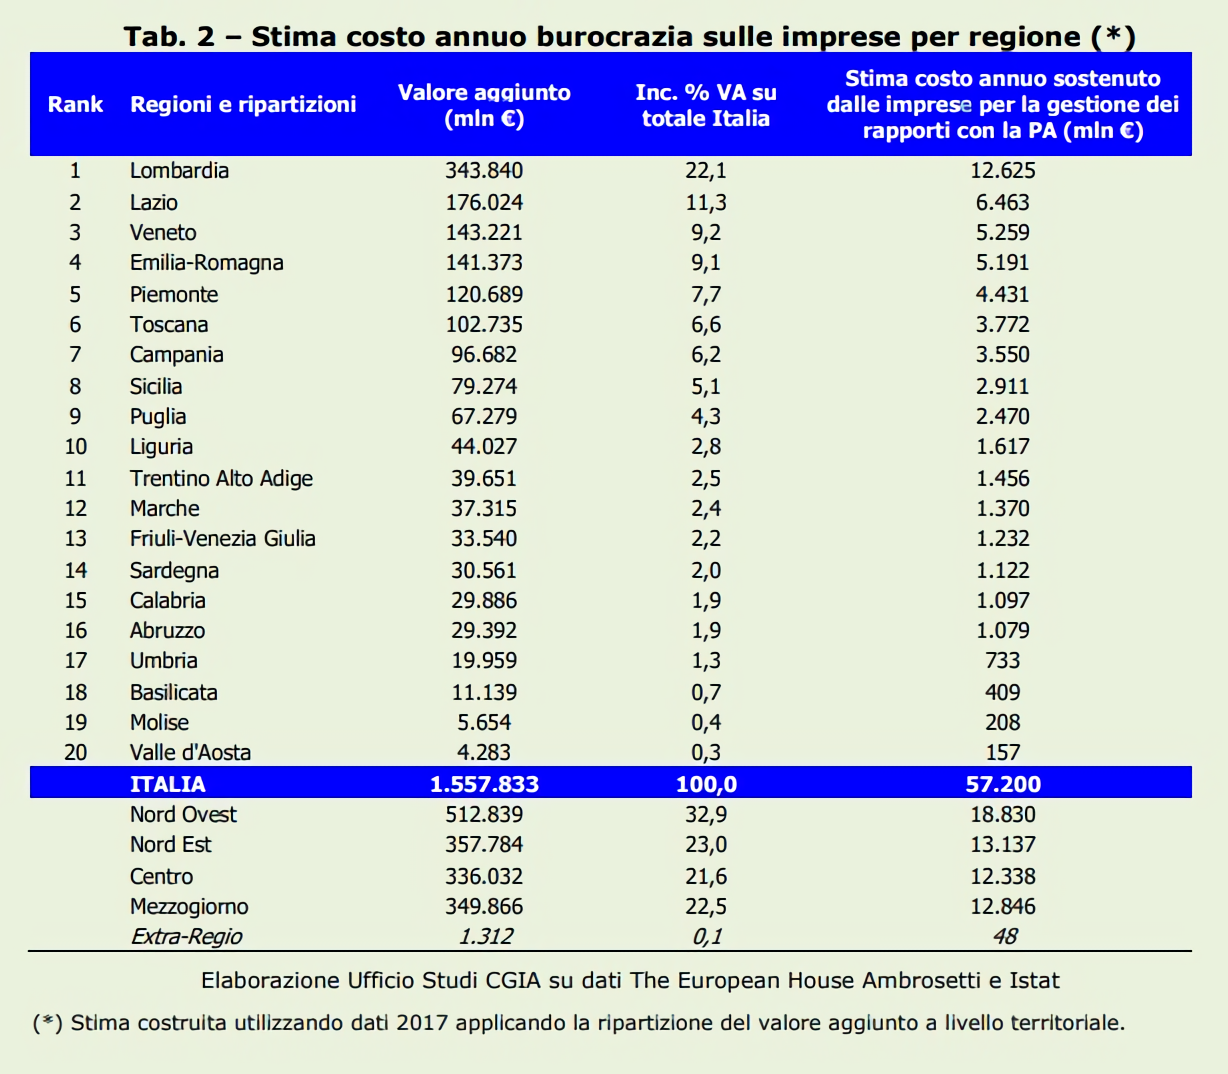
\includegraphics[width=\textwidth]{buro2.png}
			% https://www.identitafutura.it/burocrazia-allitaliana/
		\end{figure}
		\column{0.35\textwidth}
		% aggiungere qualcosa riguardo l'eccessiva burocrazia
		% si parli del miglior utilizzo dei sistemi informatici
		% un processo di efficace sbur. richiede l'attuazione di un piano di digitaliz.
		In Italia il peso dell'\textbf{eccessiva} e \textbf{confusionaria burocrazia} sulle imprese è estremo.
		Una delle priorità per il rilancio dell'economia è la \textbf{sburocratizzazione} \href{https://www.dire.it/26-03-2020/439491-coronavirus-ed-economia-il-peso-della-burocrazia-in-italia-e-un-problema-maledettamente-serio/}{[Dire.it, 2020]},
		processo che richiede un piano di \textbf{digitalizzazione}.	
	\end{columns}
\end{frame}

\begin{frame}
	\frametitle{Digitalizzazione e Recovery Fund}
	È in atto, negli ultimi anni, un piano di \textbf{digitalizzazione} della \textbf{Pubblica Amministrazione}.
	%Esso mira all'evoluzione tecnologica di tutte le sue mansioni e alla creazione
	%di portali web per il cittadino.
	L'esigenza di questa trasformazione si è fatta sentire anche da parte
	dell'\textbf{Unione Europea}, che con il \textbf{Recovery Fund}
	ci sta fornendo i fondi per attuarla, ben \textbf{11,75 milioni di euro} \\ \href{https://www.altalex.com/documents/news/2021/05/06/transizione-digitale-pubblica-amministrazione}{[Altalex.com - M. Poccu, 2021]}.
	\medskip
	% digitalizzazione PA
	% serve immagine
	% evocare quanto si spende per la burocrazia
	\begin{figure}
		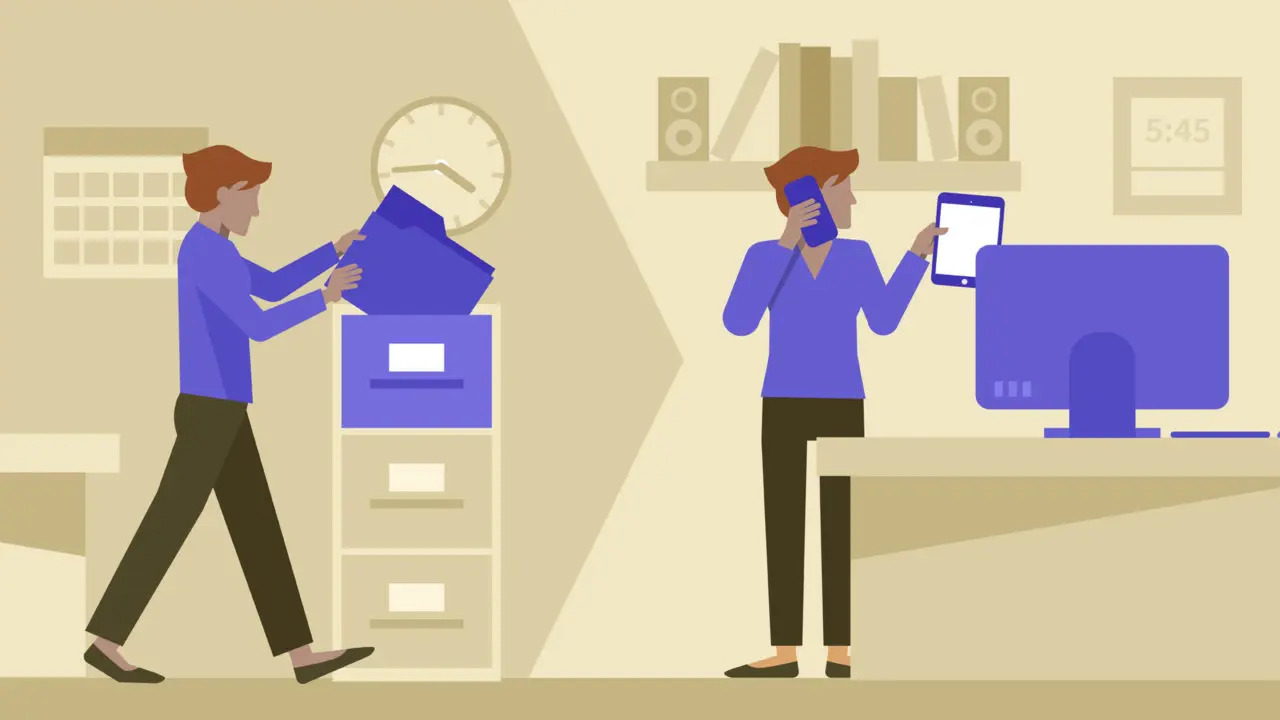
\includegraphics[width=0.55\textwidth]{digitalizzazione.jpg}
		% https://www.agendadigitale.eu/documenti/digitalizzazione-della-pa-in-italia-la-strategia-delle-tre-c/
	\end{figure}
\end{frame}

\section{L'obiettivo}
\begin{frame}
	\frametitle{L'obiettivo}
	Nell'adottare \textbf{tecniche digitali} per gestire \textbf{documenti burocratici} è fondamentale
	garantire che l'\textbf{autenticità} di tali file possa essere \textbf{verificata in modo affidabile}
	anche dai terzi a cui questi documenti sono stati \textbf{condivisi}.\\
	Considerando questo problema possiamo indicare dei sistemi evoluti che possono
	fornirci tale supporto: i \textbf{Version Control System} e la \textbf{blockchain}.
\end{frame}

%sicuramente la digit. la cui autenticità possa essere verificata in modo affidabile elemento fondamentale
% questa tesi si propone di proporre un sistema software che risponda a questa necessità.
% considerando questo prob. oggigiorno abbiamo sistemi evoluti chiamati vcs e blockchain

\begin{frame}
	\frametitle{Stato dell'arte}
	\begin{longtable}{@{}lcc@{}}
		\toprule
		\textbf{Proprietà} & \multicolumn{1}{l}{\textbf{Version Control Systems}} & \multicolumn{1}{l}{\textbf{Blockchain}} \\* \midrule
		\endfirsthead
		%
		\endhead
		%
		\bottomrule
		\endfoot
		%
		\endlastfoot
		%
		Condivisione    & 
\includegraphics[width=0.05\textwidth]{joy.png}   & 
\includegraphics[width=0.05\textwidth]{joy2.png} \\
		Tracciabilità  & 
\includegraphics[width=0.05\textwidth]{joy.png}   & 
\includegraphics[width=0.05\textwidth]{joy2.png} \\
		Autenticità  & 
\includegraphics[width=0.05\textwidth]{sad2.png}         & 
\includegraphics[width=0.05\textwidth]{joy2.png} \\
		Integrità    & 
\includegraphics[width=0.05\textwidth]{sad2.png}         & 
\includegraphics[width=0.05\textwidth]{joy2.png} \\
		Efficienza   & 
\includegraphics[width=0.05\textwidth]{joy2.png} & 
\includegraphics[width=0.05\textwidth]{sad2.png}         \\
		Flessibilità & 
\includegraphics[width=0.05\textwidth]{joy2.png} & 
\includegraphics[width=0.05\textwidth]{sad.png}       \\
		Costi        & 
\includegraphics[width=0.05\textwidth]{joy2.png}         & 
\includegraphics[width=0.05\textwidth]{sad2.png} \\* \bottomrule
	\end{longtable}
\end{frame}

\begin{frame}
	\frametitle{Git}
	% pushare che git è il software che è
	% per lo sviluppatore come la penna
	% per lo scrittore
	% scrivere che è opensource
	\begin{columns}[T]
		\column{0.99\textwidth}
		\textbf{Git} è il Version Control System (\textbf{VCS}) \\
		distribuito più diffuso al mondo. \\
		Software \textbf{Open Source} e gratuito,\\ agevola la gestione \textbf{distribuita} di insiemi\\di file e directory. \\
		Un VCS considera tali insiemi unità chiamate \textbf{repository}.\\
		Git ci permette di:
		\begin{itemize}
			\item \textbf{Tracciare} le modifiche in una repository.
			\item \textbf{Ripristinare} le repository ad uno stato precedente.
			\item \textbf{Condividere} le repository con il loro storico dei cambiamenti.
		\end{itemize}
		e molto altro\dots
		\column{0.01\textwidth}
		\hspace*{-2cm}
		
\includegraphics[width=2cm]{figures/git.png}
	\end{columns}

\end{frame}

\begin{frame}
	\frametitle{Git - Un po' di numeri}
	% pushare che git è il software che è
	% per lo sviluppatore come la penna
	% per lo scrittore

	\begin{columns}
		\column{0.5\textwidth}
		\begin{figure}
			\centering
			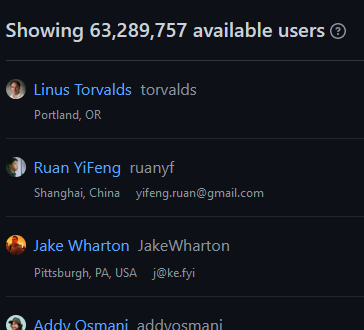
\includegraphics[width=0.8\textwidth]{users.png}
			% https://www.identitafutura.it/burocrazia-allitaliana/
		\end{figure}
		\column{0.5\textwidth}
		\begin{figure}
			\centering
			\bigskip\bigskip
			\hspace*{-1cm}
			
\includegraphics[width=\textwidth]{numberrepo.png}
			% https://www.identitafutura.it/burocrazia-allitaliana/
		\end{figure}
	\end{columns}
	\begin{figure}
		\centering
		
\includegraphics[width=\textwidth]{companies.png}
		% https://www.identitafutura.it/burocrazia-allitaliana/
	\end{figure}
\end{frame}

\begin{frame}
	\frametitle{Blockchain}
	La \textbf{blockchain} è un registro di
	contenitori immutabili chiamati \textbf{blocchi}, collegati l'uno all'altro come in una
	\textbf{catena} grazie a \textbf{metodi crittografici}.
	Essa è:
	\begin{itemize}
		\item \textbf{Immutabile}.
		\item \textbf{Distribuita}.
		\item \textbf{Estremamente sicura}.
	\end{itemize}
	Grazie a ciò è l'ideale per effettuare \textbf{verifiche d'integrità}.
	\begin{figure}
		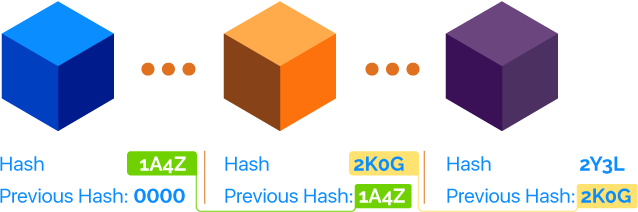
\includegraphics[width=0.65\textwidth]{figures/blockchain.png}
		% https://rubygarage.org/blog/how-blockchain-works
	\end{figure}
	\pause
	È alla base delle reti di criptovalute, come \textbf{Ethereum},
	su cui si possono anche costruire applicazioni decentralizzate con gli
	\textbf{Smart Contract}.
\end{frame}

%\begin{frame}
%	\frametitle{Perché blockchain?}
%	L'utilizzo della blockchain nel progetto è giustificato da:
%	\begin{itemize}%[<+->]
%		\item \textbf{Immutabilità} \(\rightarrow\) Garantisce integrità dei dati.
%		\item \textbf{Decentralizzazione} \(\rightarrow\) Resistenza al Single Point Of Failure.
%		\item \textbf{Disintermediazione} \(\rightarrow\) Eliminazione di \emph{middle-men} e dei loro costi.
%		\item \textbf{Validazione \emph{peer-to-peer}} \(\rightarrow\) Potere distribuito.
%	\end{itemize}
%\end{frame}

%spostare a dopo
% introdurre SU e poi ci va l'hash
% Autenticazione con blockchain
% parto da repo con solo documento -> vogliamo dargli garanzia
% -> calcolo hash -> salvo hash su blockchain ->
% -> mi prendo il timestamp
% si chiama batching

\begin{frame}
	\frametitle{Funzioni crittografiche di hashing}
	Funzione che \textbf{associa},
	a una qualsiasi sequenza \(m\) di lunghezza arbitraria in input, una sequenza
	in output \(h(m)\) di lunghezza costante,
	garantendo alcune proprietà che la rendono
	\emph{crittograficamente sicura}.
	Sono estremamente impiegate per effettuare \textbf{controlli di integrità sui file}.
	\begin{figure}
		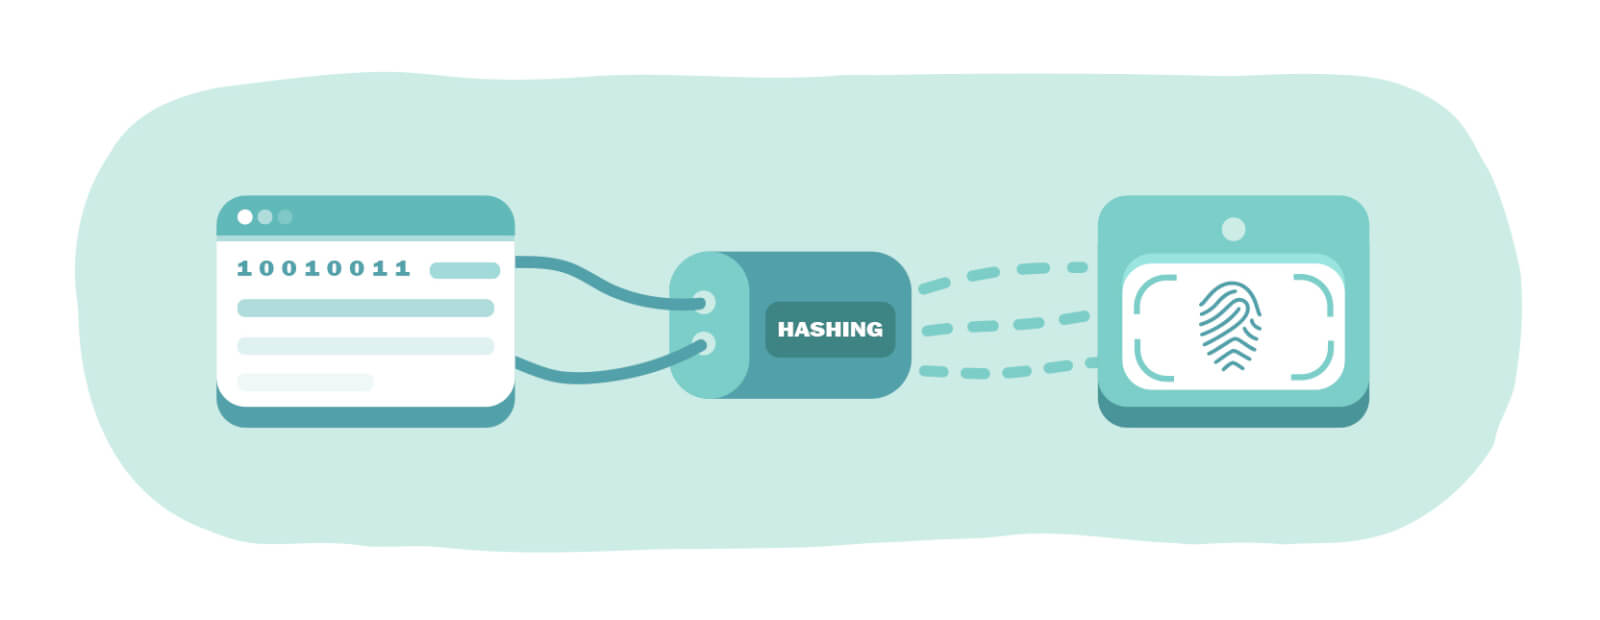
\includegraphics[width=0.85\textwidth]{figures/hashing.jpg}
	\end{figure}
\end{frame}


\begin{frame}
	\frametitle{Verifica d'integrità/autenticità con blockchain}
	\begin{columns}
		\column{0.5\textwidth}
		\begin{figure}
			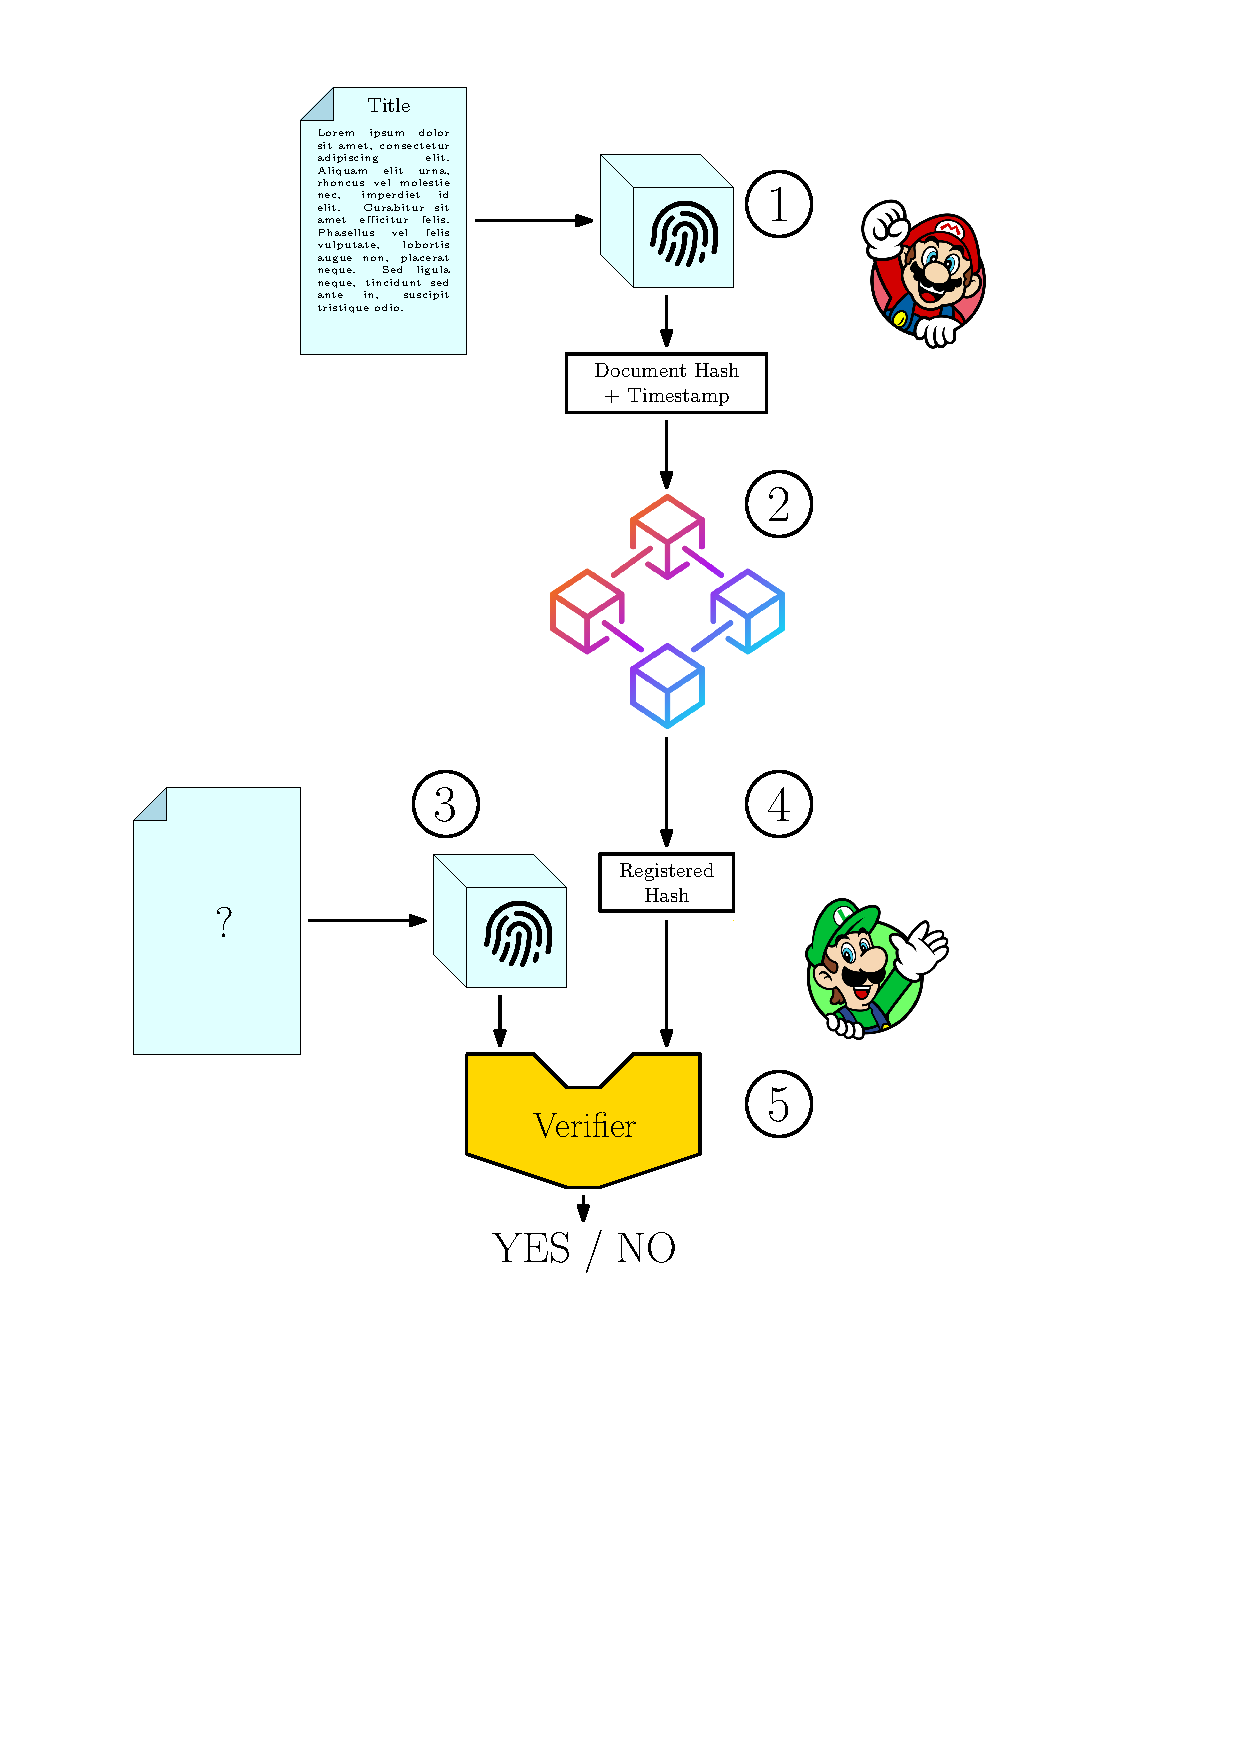
\includegraphics[width=\textwidth]{figures/hashsaving2.pdf}
		\end{figure}
		\column{0.5\textwidth}
		\begin{enumerate}
			\item Calcolo \textbf{impronta digitale} del documento tramite una \textbf{funzione crittografica di hashing}.
			\item Registrazione impronta su \textbf{blockchain}.
			\item Calcolo \textbf{impronta digitale} del documento da verificare.
			\item Reperimento dell'\textbf{impronta} da blockchain.
			\item \textbf{Confronto delle impronte}.
		\end{enumerate}
	\end{columns}
\end{frame}

% prendo documento con punto interrogativo e txhash

\begin{frame}
	\frametitle{Costo della blockchain}
	Non possiamo però effettuare un'operazione di registrazione su blockchain per \textbf{ogni singolo file}
	e nemmeno per \textbf{ogni singola repository}, sarebbe troppo \textbf{costoso}.
	La soluzione è l'utilizzo di \textbf{accumulatori crittografici}:
	strumenti che \textbf{calcolano} in modo efficiente \textbf{l'impronta digitale}
	di una \textbf{collezione} di file.
	% tempo di verifica cresce ma noi usiamo strutture bilanciate
	\medskip
	\begin{figure}
		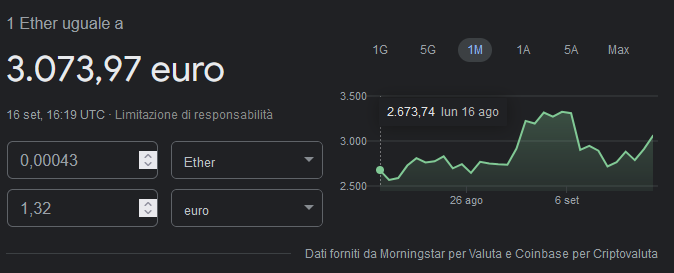
\includegraphics[width=0.85\textwidth]{figures/costo.png}
	\end{figure}
\end{frame}

\section{Il problema affrontato}
\begin{frame}
	\frametitle{Il problema affrontato}
	Realizzare uno \textbf{software} che combini \textbf{Git} con una \textbf{blockchain} e sia in grado di:
	\medskip
	\begin{columns}
		\column{0.33\textwidth}
		\centering
		\begin{figure}
			
\includegraphics[width=0.7\textwidth]{figures/fingerprint.png}
		\end{figure}
		\textbf{Salvare} l'\emph{impronta digitale} di
		repository su
		blockchain
		\column{0.33\textwidth}
		\centering
		\begin{figure}
			
\includegraphics[width=0.7\textwidth]{figures/folder_zip.png}
		\end{figure}
		\textbf{Esportare} sottoinsiemi
		di repository verificabili
		\column{0.33\textwidth}
		\centering
		\begin{figure}
			
\includegraphics[width=0.7\textwidth]{figures/verify.png}
		\end{figure}
		\textbf{Verificare} l'integrità
		di singoli file e repository
	\end{columns}
\end{frame}

\section{Il Software PineSU}
\begin{frame}
	\frametitle{Il Software PineSU}
	\begin{columns}
		\column{0.7\textwidth}
		\textbf{PineSU} è un software \textbf{Javascript} che sfrutta il run-time \textbf{Node.js}. \\
		\smallskip
		L'applicazione si basa sul concetto di
		\textbf{Storage Unit} (SU): \textbf{repository Git} dotate di speciali metadati. \\
		%\smallskip
		%Queste SU sono le unità su cui effettueremo le singole
		%operazioni, eccetto la registrazione su blockchain che si svolgerà
		%collettivamente con l'ausilio di accumulatori crittografici. 
		\column{0.3\textwidth}
		\centering
		\begin{figure}
			
\includegraphics[width=\textwidth]{figures/favicon.png}
		\end{figure} 
	\end{columns}
\end{frame}

\begin{frame}[fragile]
	\frametitle{Storage Unit}
	\begin{columns}
		\column{0.59\textwidth}
		\centering
		\begin{figure}
			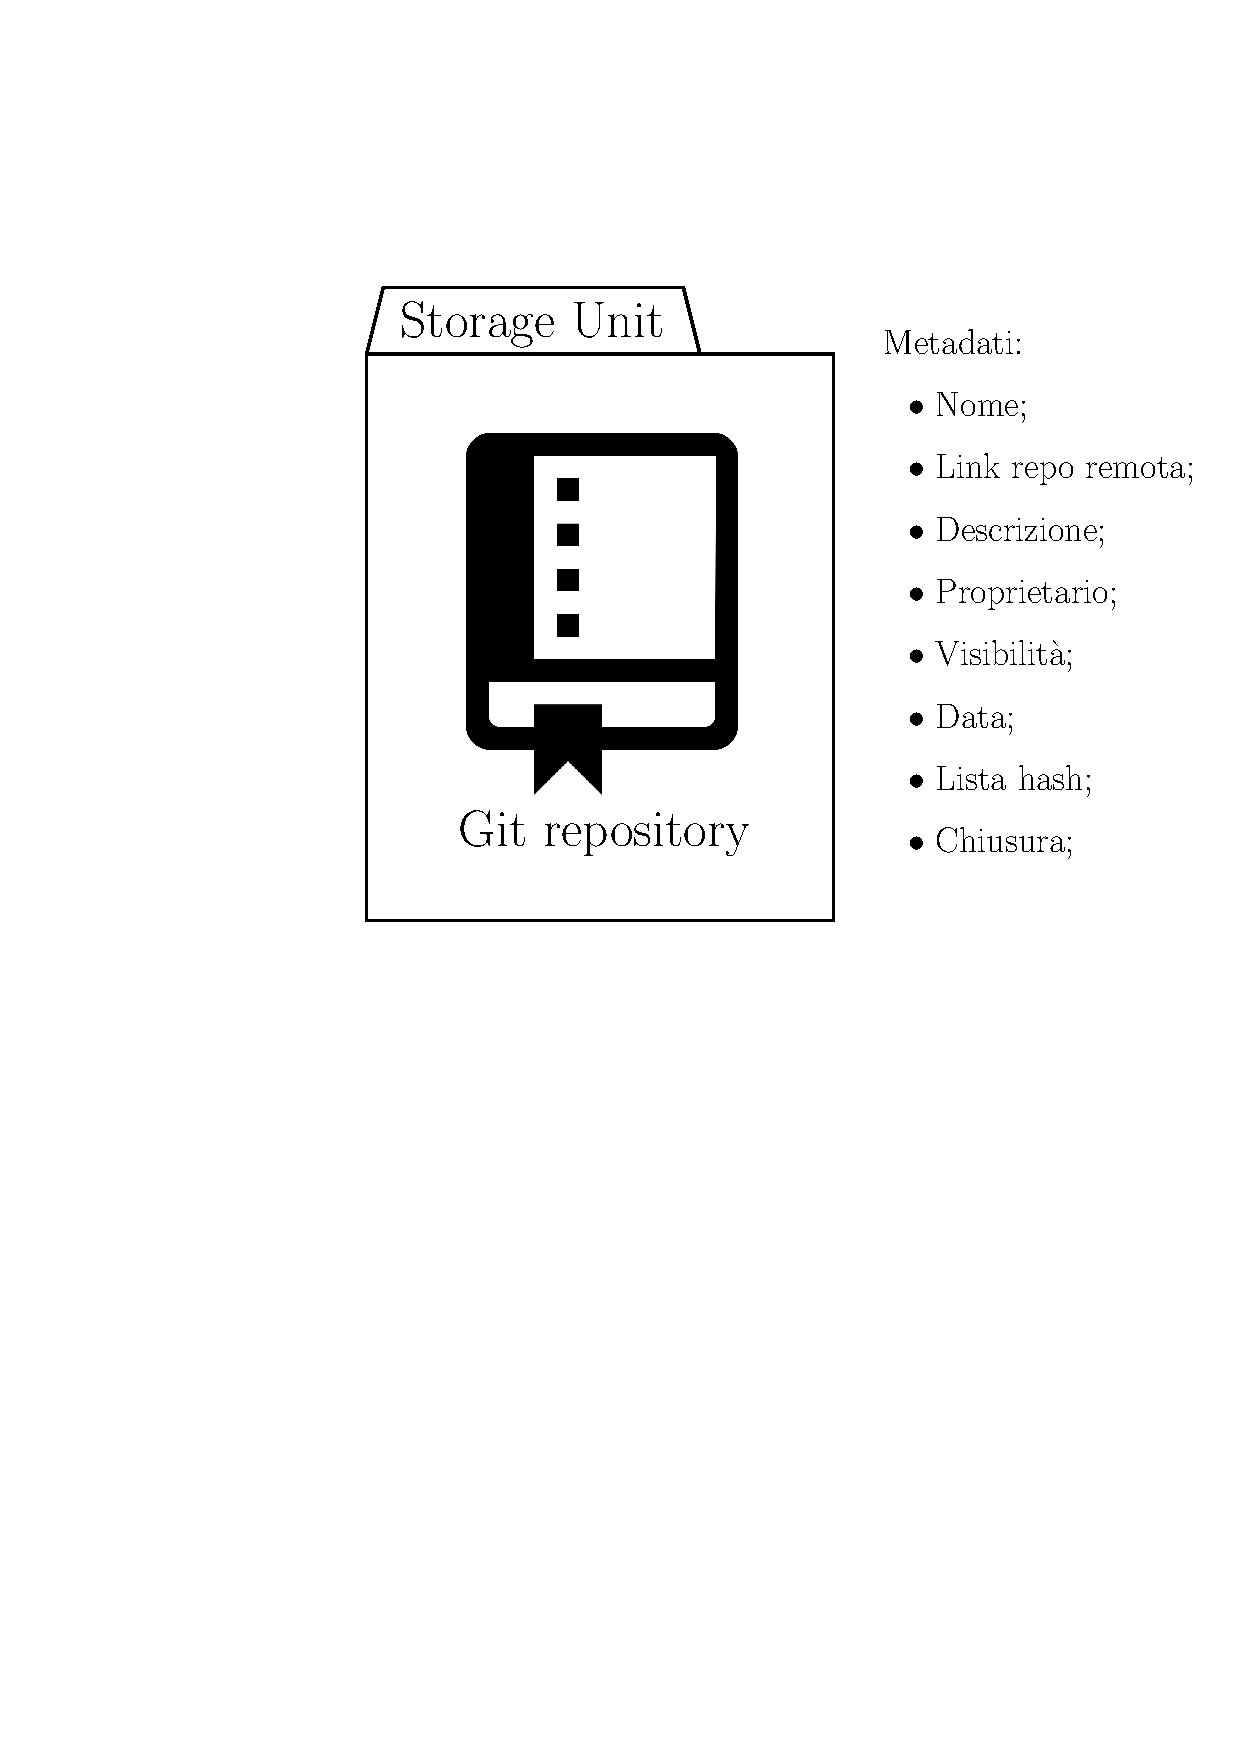
\includegraphics[width=\textwidth]{figures/repo.pdf}
		\end{figure}
		\column{0.41\textwidth}
		\vspace{0.9cm}
		\centering
		\begin{lstlisting}[language=JavaScript, numbers=none]
		|\color{blue}"name"|: "sample",
		|\color{blue}"remote"|: "github.com/
			plspeziali/sample",
		|\color{blue}"description"|: "example",
		|\color{blue}"visibility"|: "public",
		|\color{blue}"date"|: "2021-08-18",
		|\color{blue}"owner"|: "0xCF2[...]66",
		|\color{blue}"hash"|: "3837e[...]53",
		|\color{blue}"filelist"|: [
			|\textcolor{cyan}{"b/astar.js:e09[...]9b6"}|,
			|\textcolor{cyan}{"c/graph.js:539[...]1cc"}|,
			[...]],
		|\color{blue}"closed"|: false
		\end{lstlisting}
	\end{columns}
\end{frame}



\begin{frame}
	\frametitle{Workflow}
	\centering
	\begin{figure}
		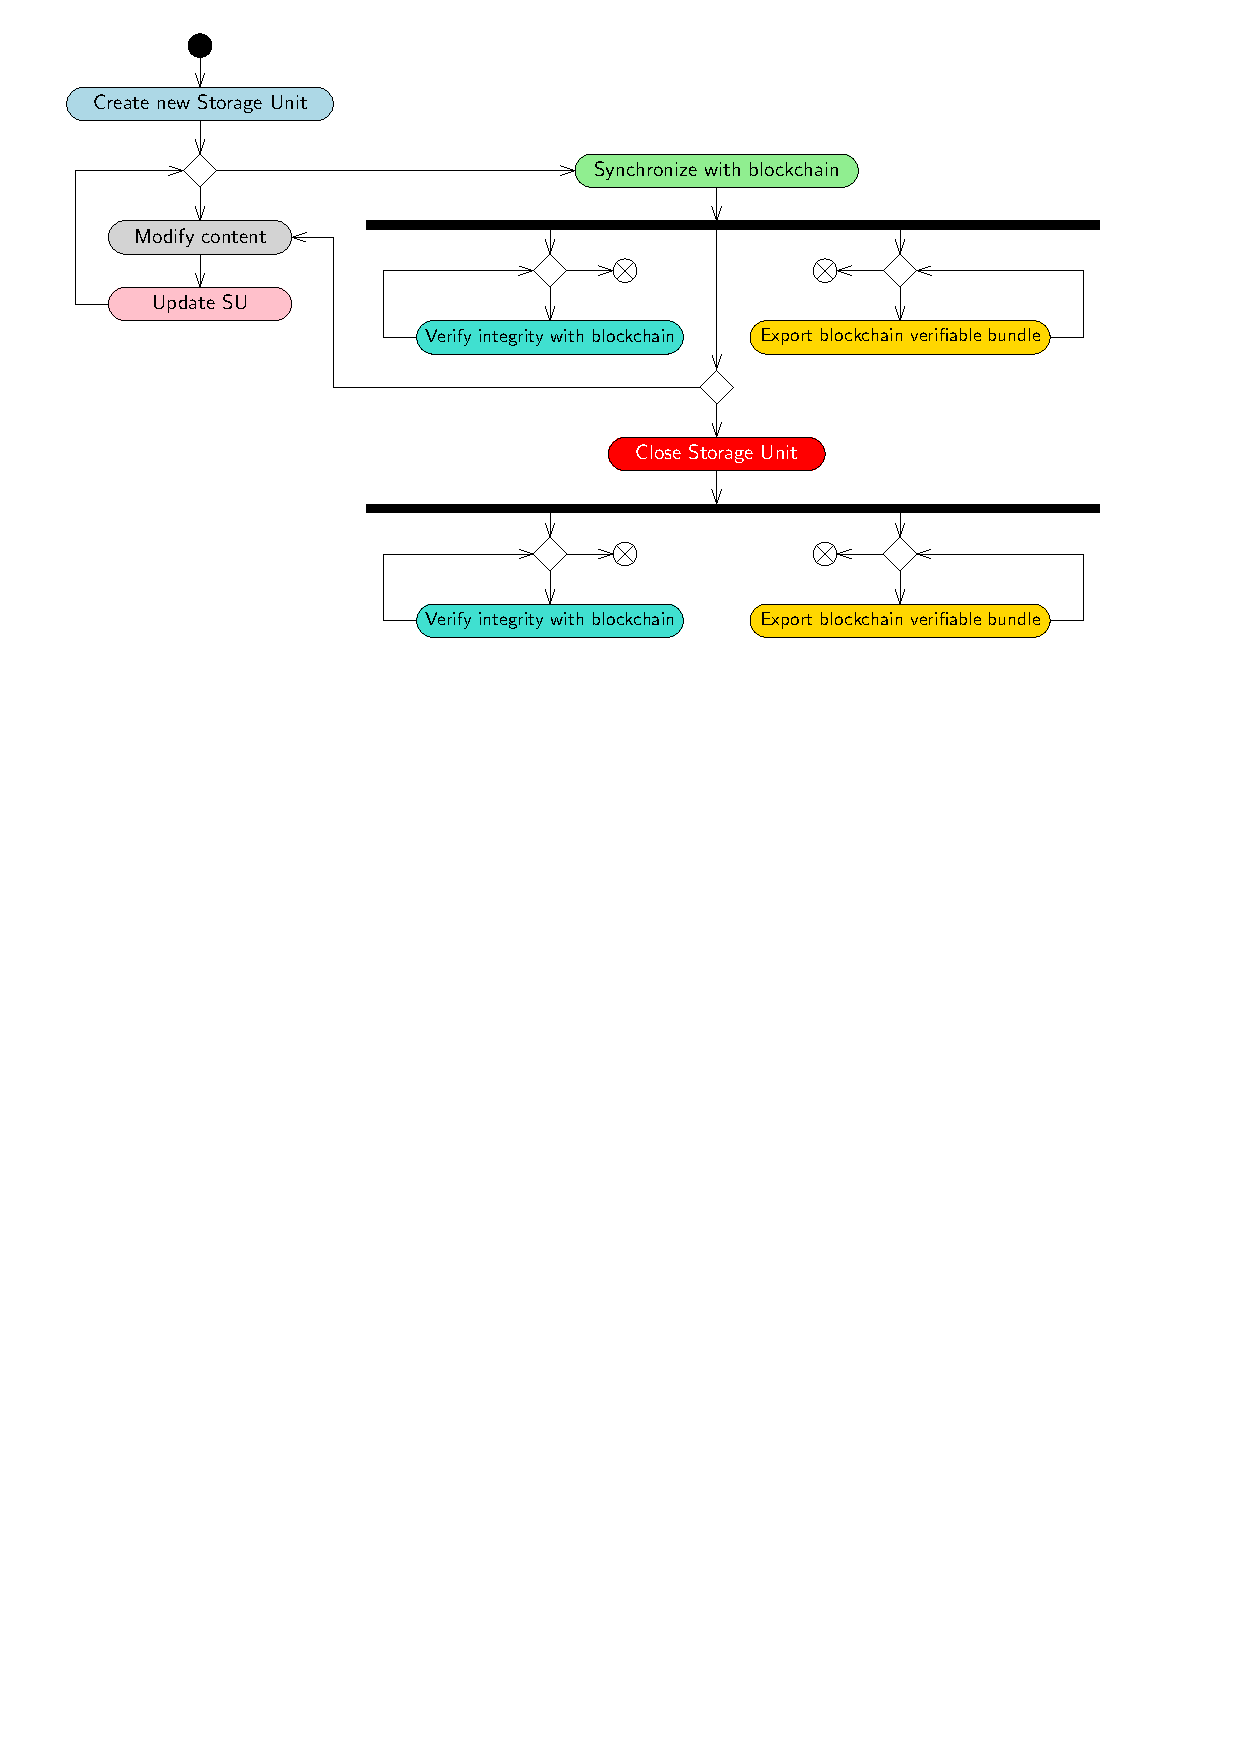
\includegraphics[width=\textwidth]{figures/activityDiag.pdf}
	\end{figure}
\end{frame}

% qua l'interfaccia

\begin{frame}
	\frametitle{Ciclo vitale di una Storage Unit}
	\centering
	\begin{figure}
		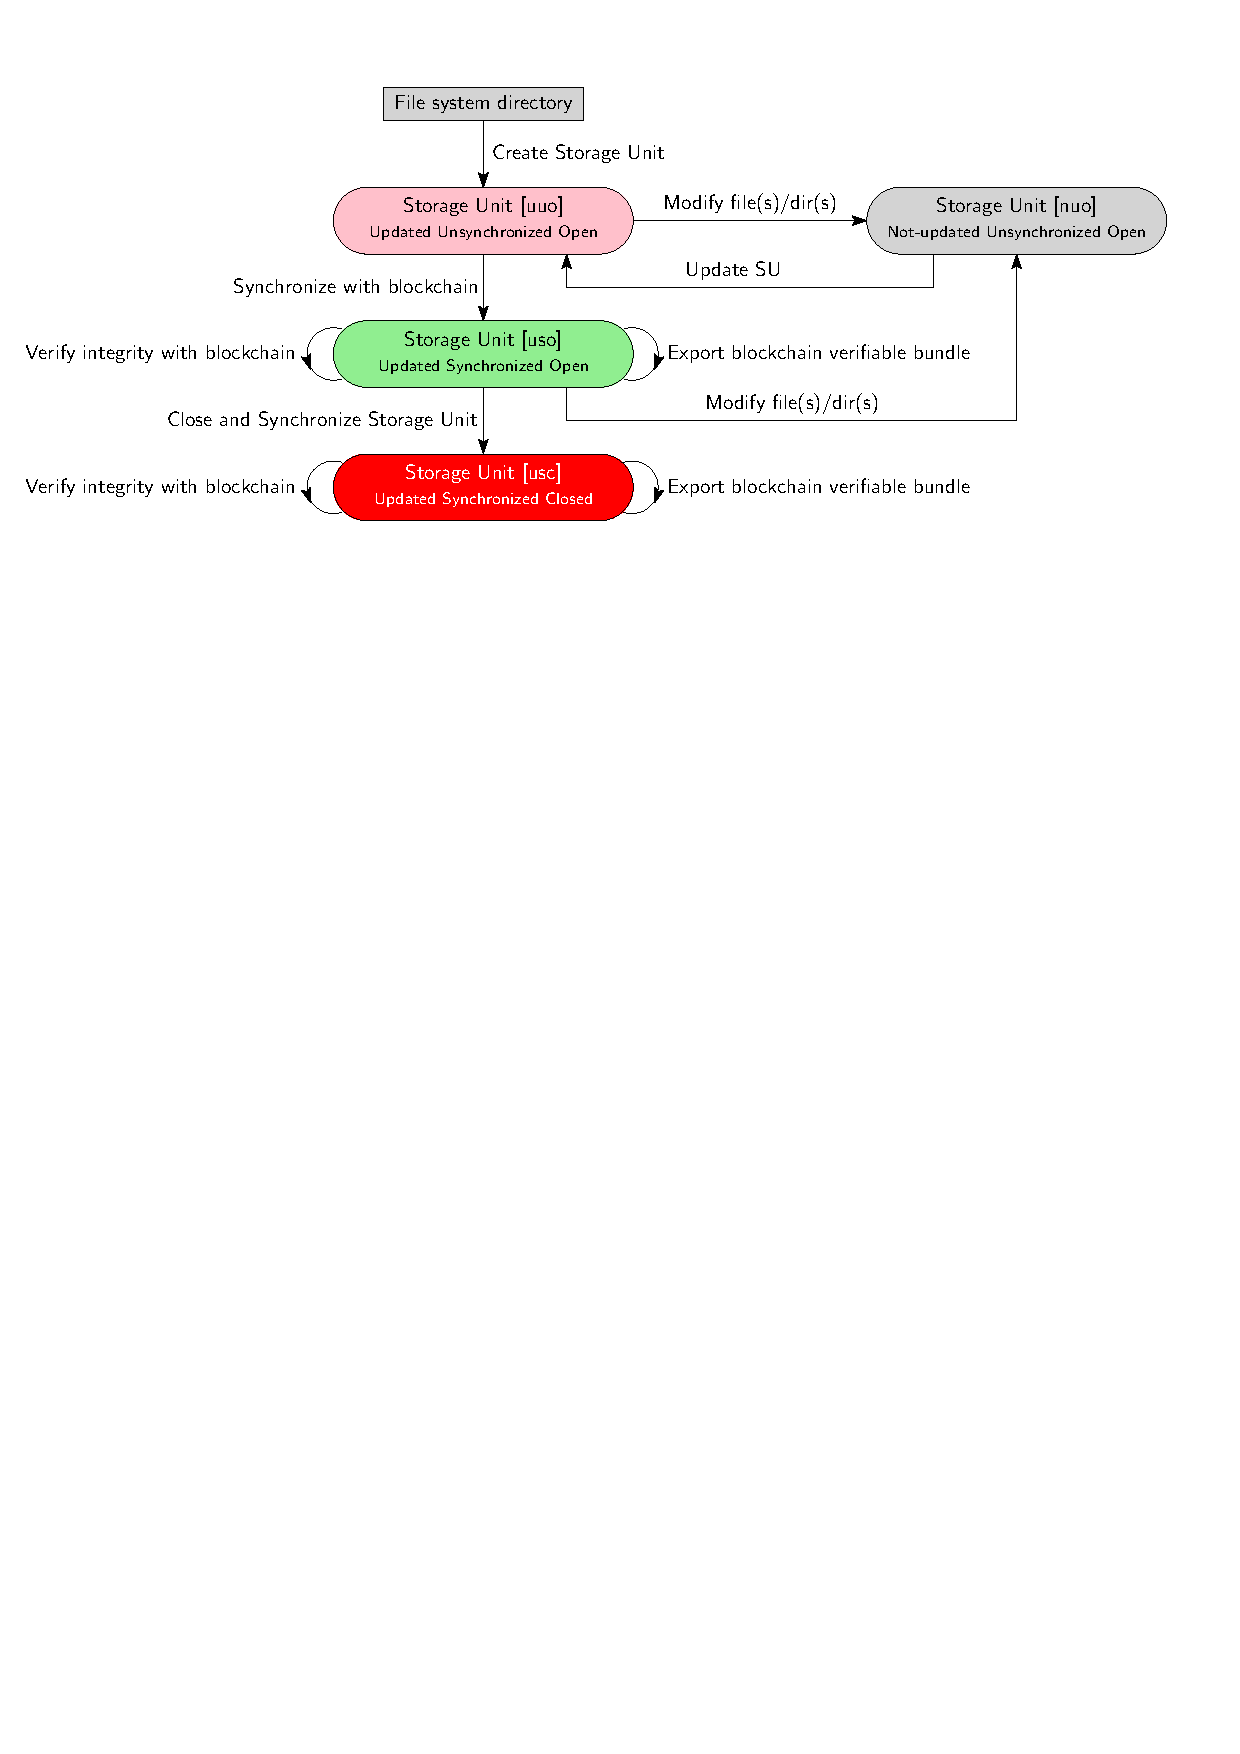
\includegraphics[width=\textwidth]{figures/stateDiag2.pdf}
	\end{figure}
\end{frame}

% è blockchain-agnostic
\begin{frame}
	\frametitle{Architettura}
	\centering
	\begin{figure}
		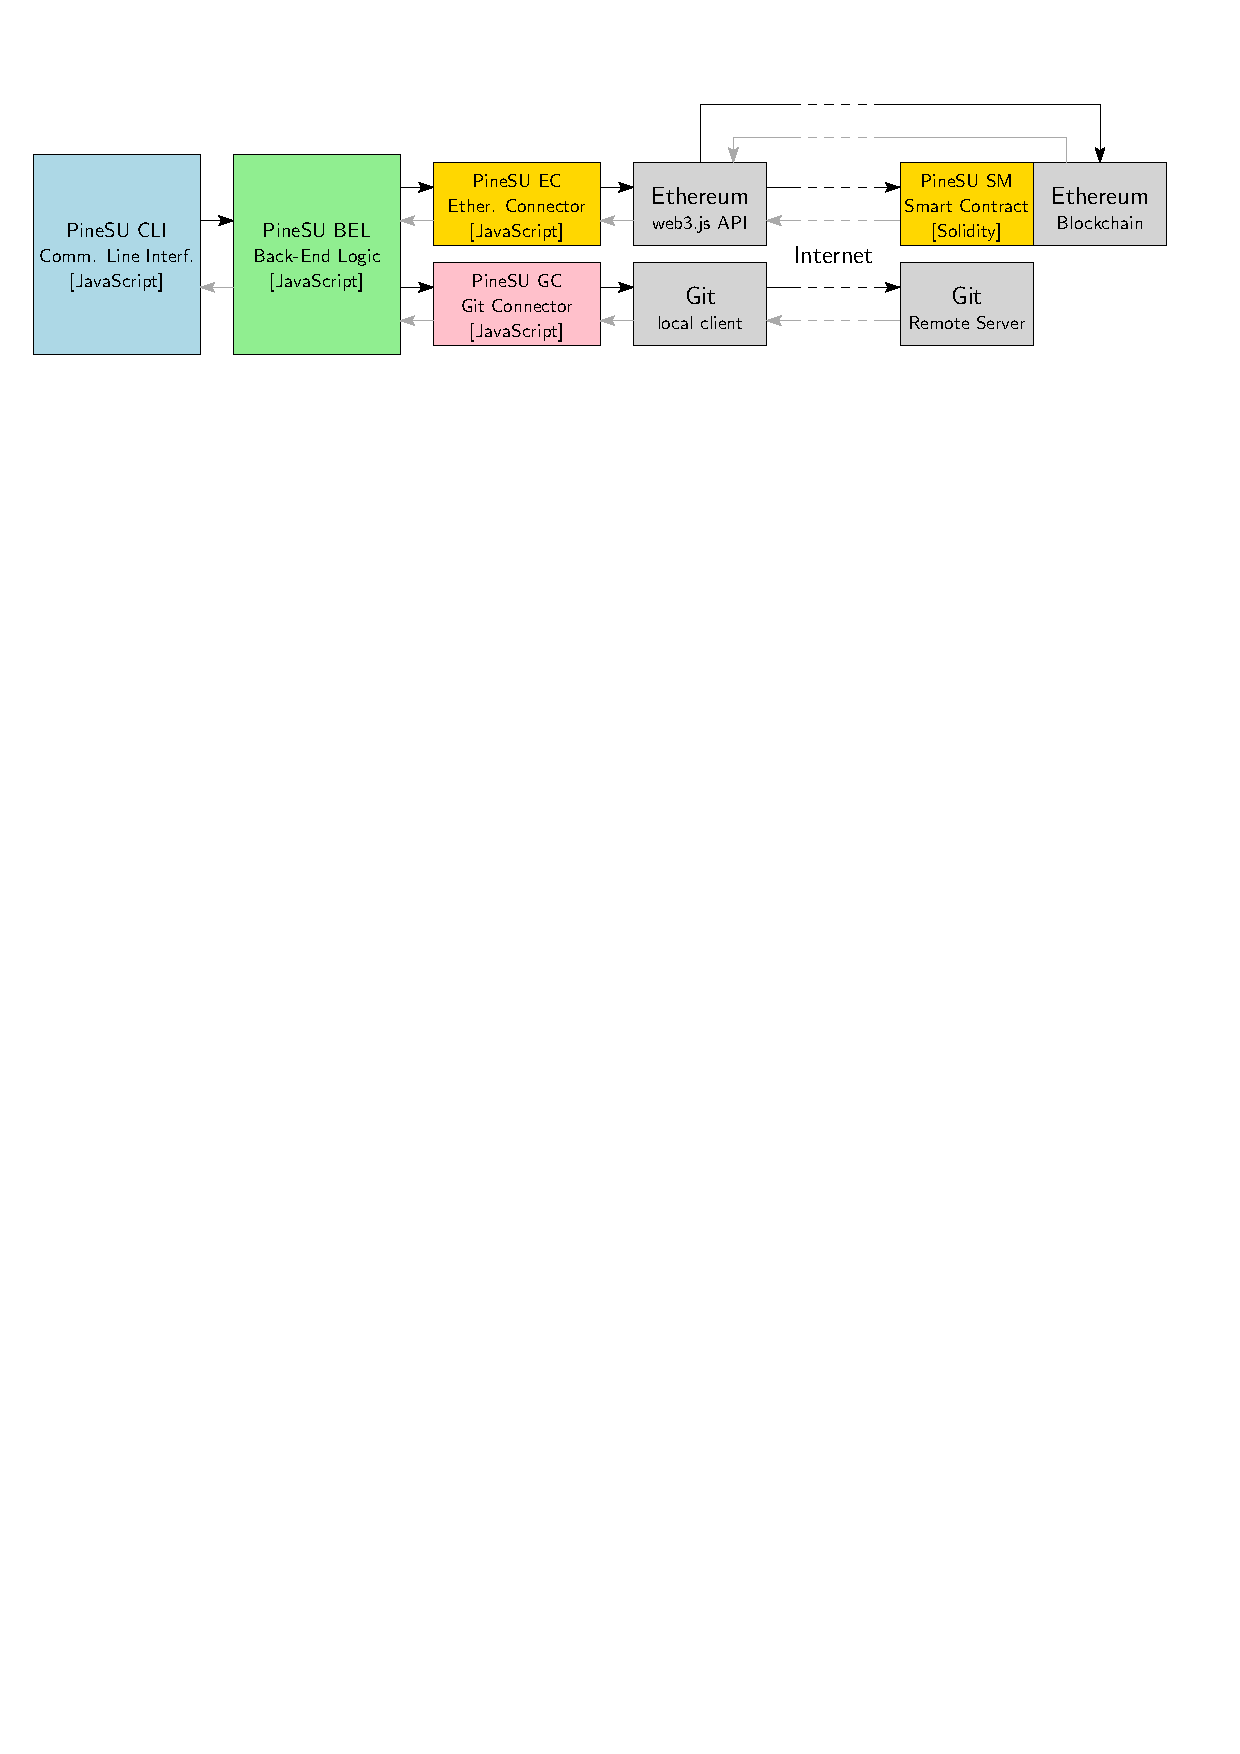
\includegraphics[width=\textwidth]{figures/pineSU-architecture.pdf}
	\end{figure}
\end{frame}

\begin{frame}
	\frametitle{Architettura (Cont.)}
	\begin{itemize}
		\item \emph{PineSU \textbf{CLI} (Command Line Interface)}: \textbf{Crea l'interfaccia utente} con cui è possibile
			interagire e \textbf{richiama le funzioni} degli altri moduli all'occorrenza.
		\item \emph{PineSU \textbf{BEL} (Back End Logic)}: Il \textbf{nucleo} di PineSU.
		\textbf{Gestisce le SU} e controlla la comunicazione con la \textbf{blockchain} e il client \textbf{Git} locale.
		\item \emph{PineSU \textbf{EC} (Ethereum Connector)}: Si interfaccia con le \textbf{API della blockchain}. 
		\item \emph{PineSU \textbf{GC} (Git Connector)}: Si interfaccia con il \textbf{client Git}. 
		\item \emph{PineSU \textbf{SM} (Smart Contract)}: Permette \textbf{registrazioni permanenti} di singole SU nella blockchain.
	\end{itemize}
\end{frame}

\begin{frame}
	\frametitle{PineSU CLI}
	\centering
	\begin{figure}
		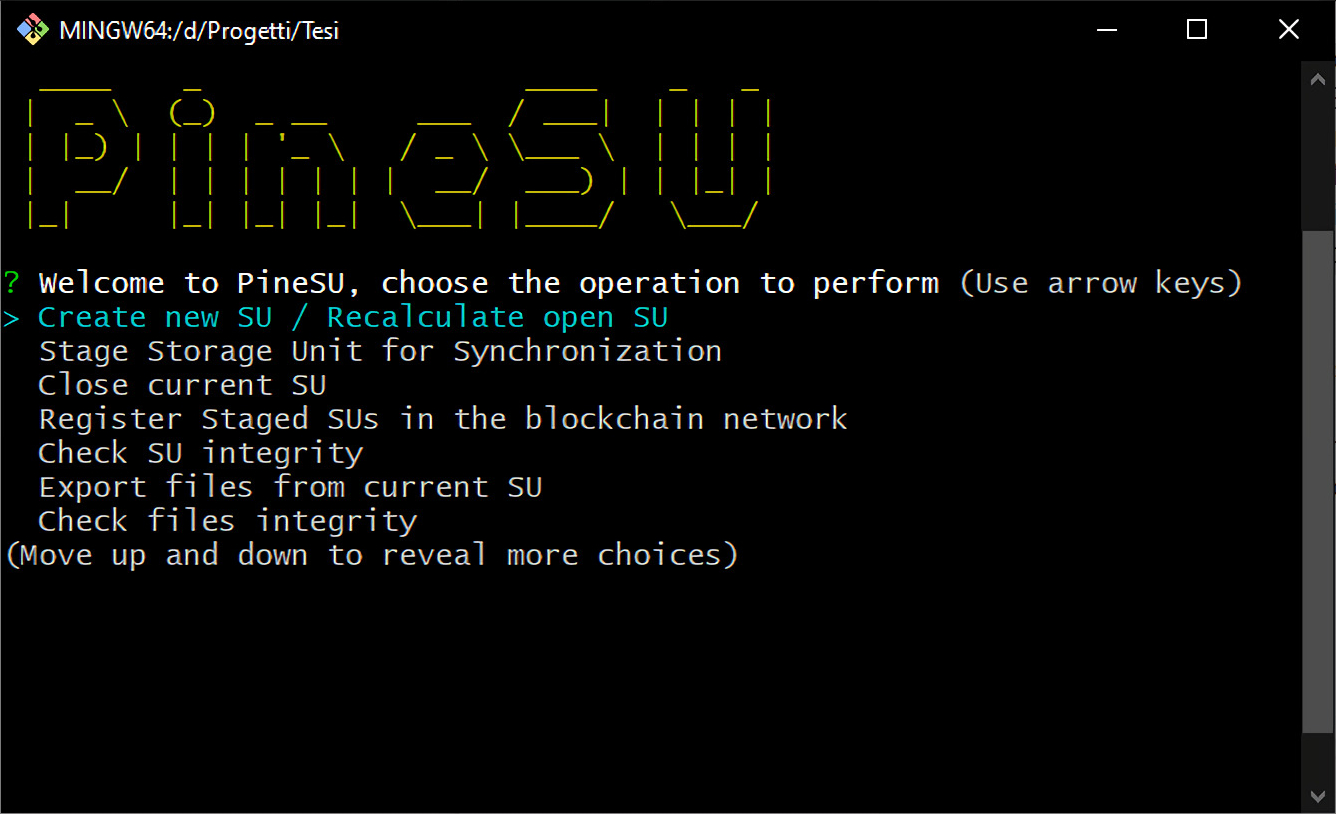
\includegraphics[width=0.95\textwidth]{figures/menu.jpg}
	\end{figure}
\end{frame}

\begin{frame}
	\frametitle{PineSU BEL}
	Il nucleo centrale che si occupa di:
	\begin{enumerate}
		\item \textbf{Gestione} dei \textbf{file descrittori}.
		\item \textbf{Gestione} degli \textbf{accumulatori crittografici}.
		\item \textbf{Comunicazione} con \textbf{Git} e \textbf{blockchain}.
	\end{enumerate}
\end{frame}

% spiega solo MC	cava SG
% togli MT

\begin{frame}
	\frametitle{Merkle Calendar}
	\begin{columns}
		\column{0.6\textwidth}
		Il \emph{Merkle Calendar (\textbf{MC})} è l'\textbf{accumulatore critografico}
		più importante di PineSU. Si tratta di un albero in cui le \textbf{foglie} sono
		i Blockchain Synchronization Point (\textbf{BSP}), istanze di
		Storage Group, a loro volta raggruppate in nodi rappresentanti
		\textbf{mesi e anni}, ciò rende i reperimenti di registrazioni passate
		più agevoli e veloci.
		\column{0.4\textwidth}
		\centering
		\begin{figure}
			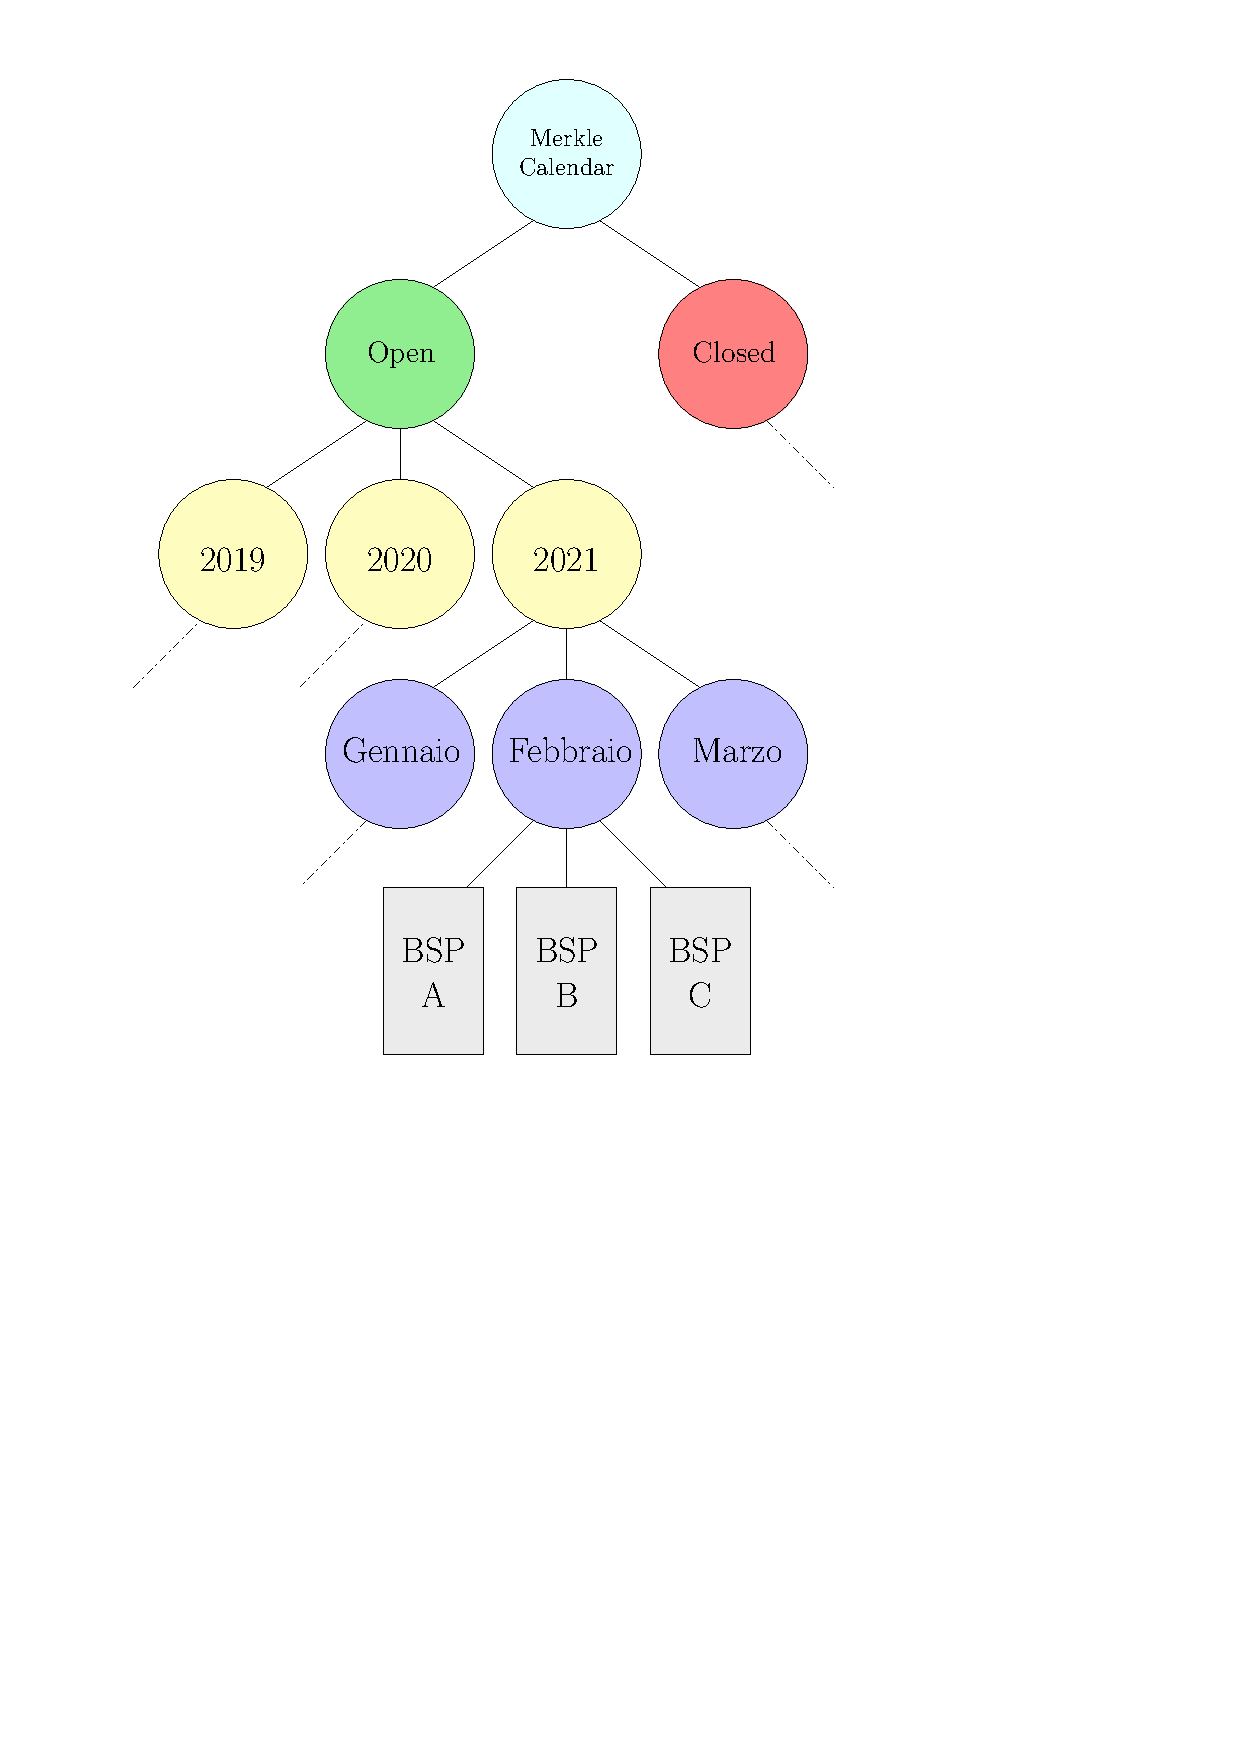
\includegraphics[width=\textwidth]{figures/mc1.pdf}
			\caption{Un Merkle Calendar}
		\end{figure} 
	\end{columns}
\end{frame}

\begin{frame}
	\frametitle{Merkle Calendar UML}
	\begin{figure}
		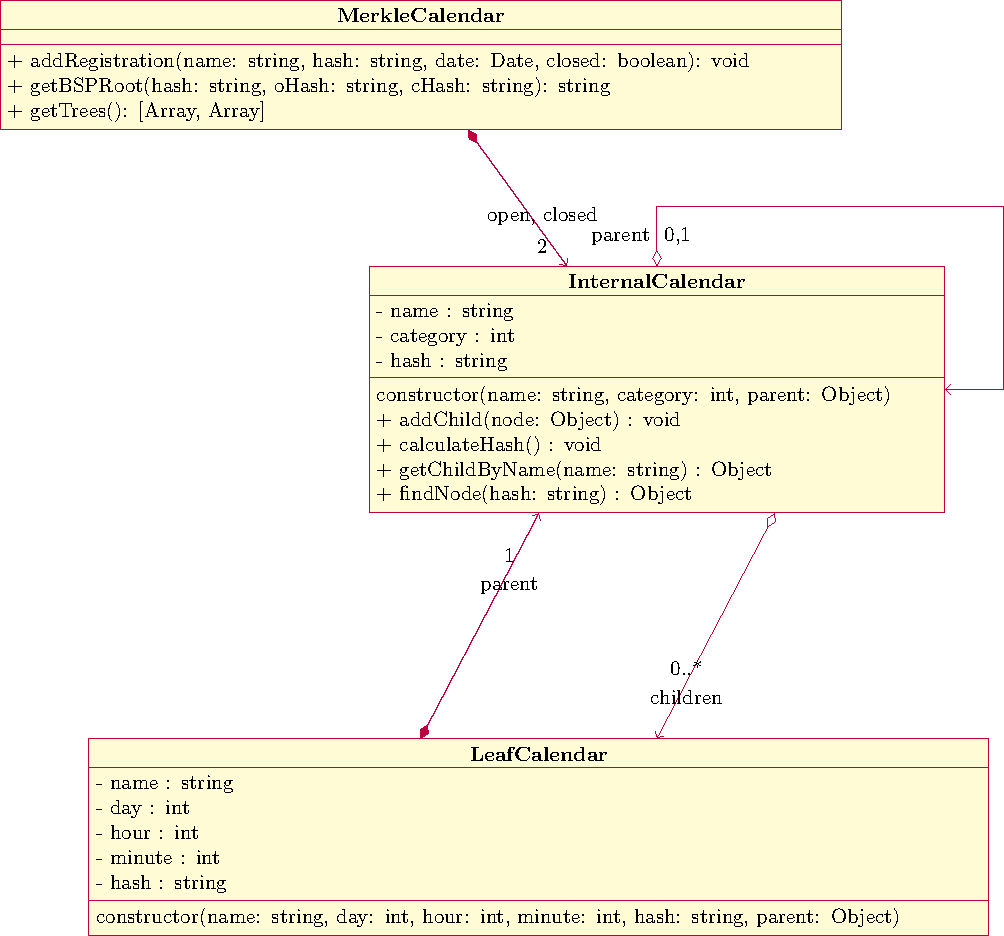
\includegraphics[width=0.75\textwidth]{figures/umlmc.pdf}
	\end{figure}
\end{frame}

\begin{frame}[fragile]
	\frametitle{Codice - Reperimento di una BSP Root}
	\begin{lstlisting}[language=JavaScript, numbers=none]
	for(let i = 0; i <= leafIndex; i++){
		leavesHash.push(monthNode.getChildByNum(i).getHash())
	}
	let newMonth = this.calculateHash(leavesHash);
	let monthsHash = new Array();
	for(let i = 0; i < monthIndex; i++){
		monthsHash.push(yearNode.getChildByNum(i).getHash())
	}
	monthsHash.push(newMonth);
	let newYear = this.calculateHash(monthsHash);
	let yearsHash = new Array();
	for(let i = 0; i < yearIndex; i++){
		yearsHash.push(yearNode.getChildByNum(i).getHash())
	}
	yearsHash.push(newYear);
	let newRoot = this.calculateHash(yearsHash)
	\end{lstlisting}
\end{frame}

\begin{frame}
	\frametitle{PineSU GC}
	\begin{figure}
		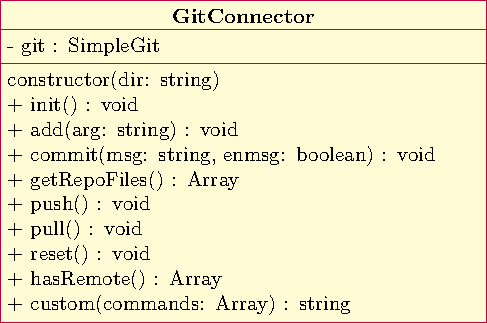
\includegraphics[width=0.85\textwidth]{figures/umlgc.pdf}
	\end{figure}
\end{frame}

\begin{frame}
	\frametitle{PineSU EC}
	\begin{figure}
		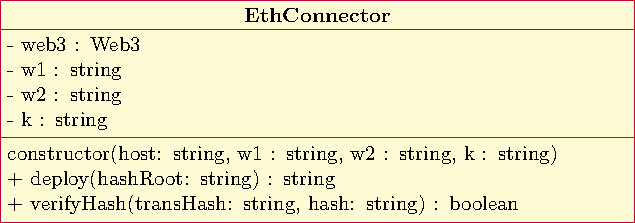
\includegraphics[width=\textwidth]{figures/umlec.pdf}
	\end{figure}
\end{frame}

\begin{frame}[fragile]
	\frametitle{Codice - Salvataggio di un hash su blockchain}
	% mettere immagine w1 -> w2 con messaggino in allegato
	\begin{lstlisting}[language=JavaScript, numbers=none]
	async deploy(hashRoot){
		const ct = await this.web3.eth.accounts
			.signTransaction({
				from: this.w1,
				to: this.w2,
				data: hashRoot,
				gas: 3000000,
			},
			this.k
		);
		const receipt = await this.web3.eth
			.sendSignedTransaction(ct.rawTransaction);
		return receipt.transactionHash;
	}
	\end{lstlisting}
	\vspace{-0.8cm}
	\begin{figure}
		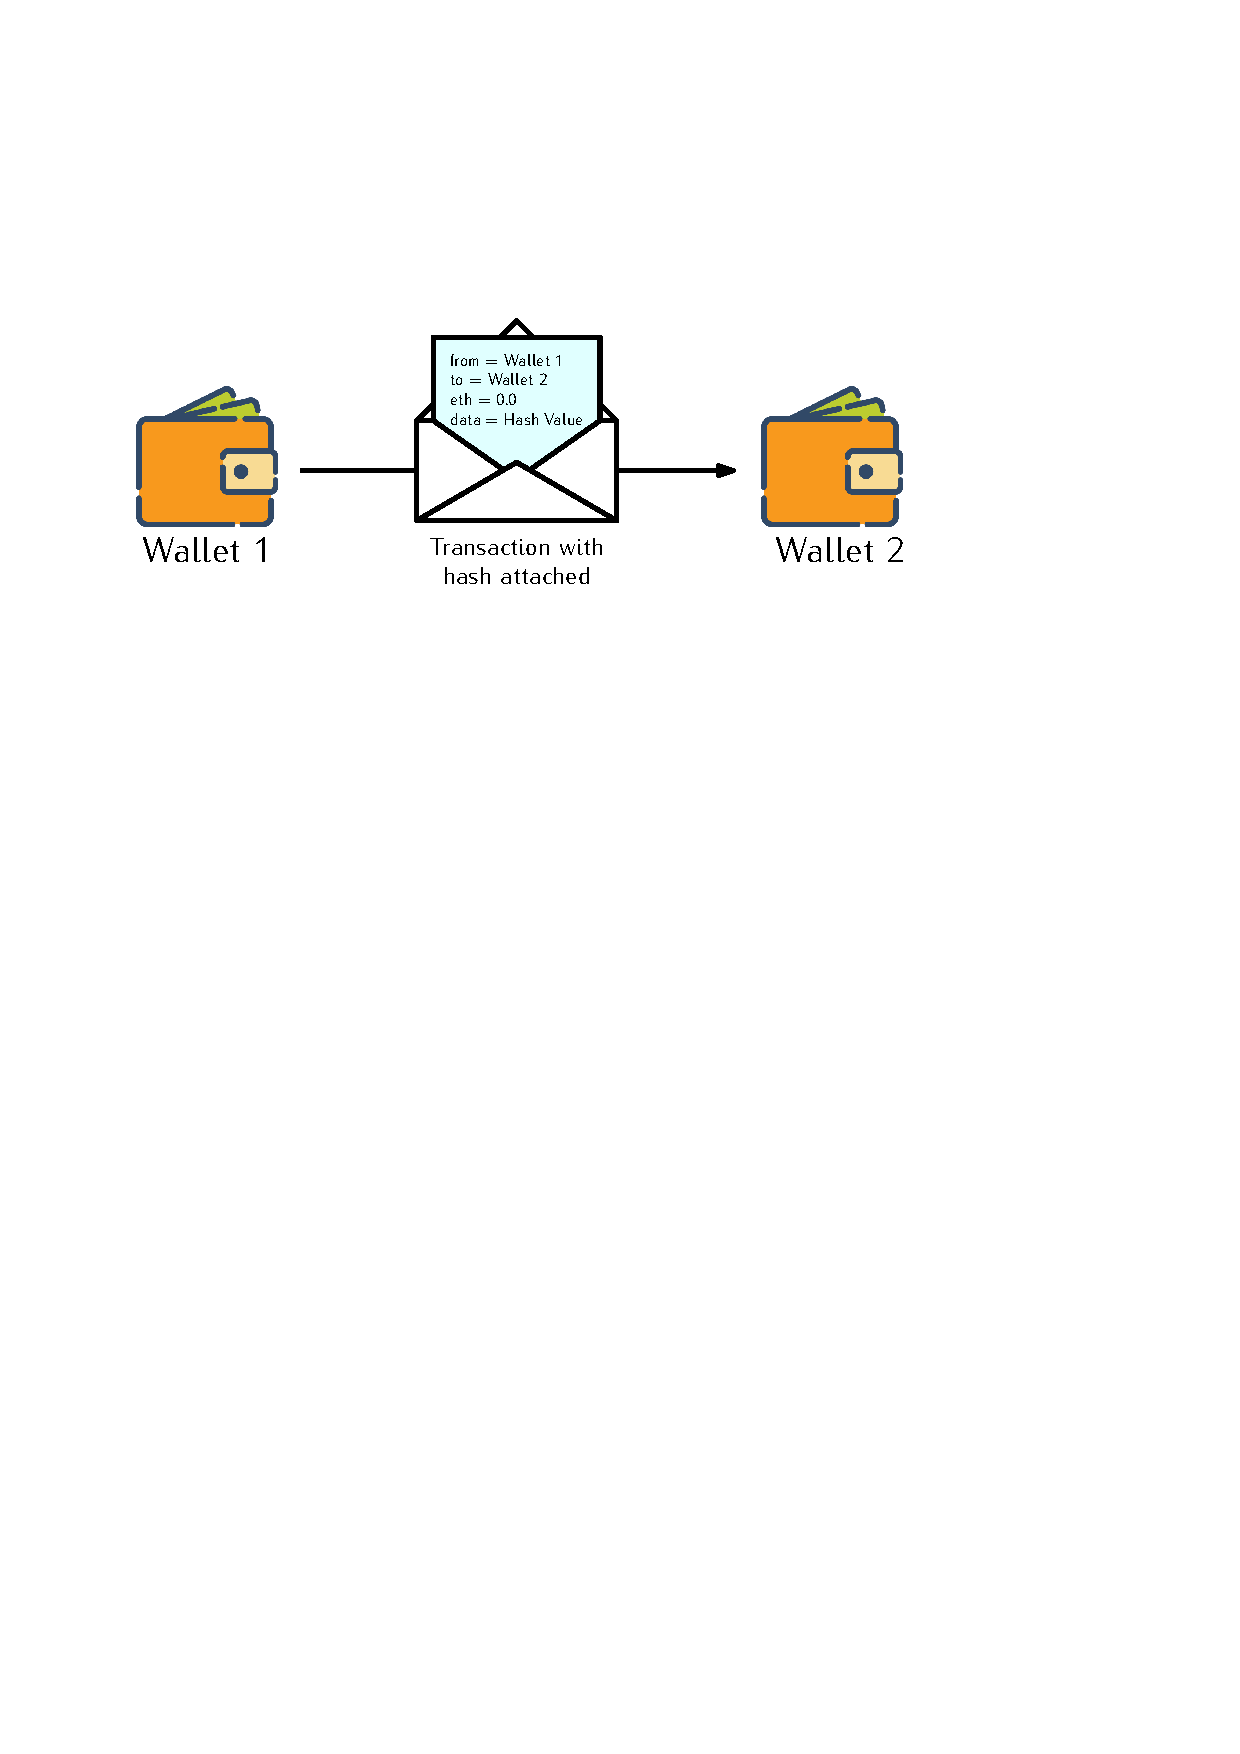
\includegraphics[width=0.7\textwidth]{figures/wallets.pdf}
	\end{figure}
\end{frame}

\begin{frame}[fragile]
	\frametitle{PineSU SM}
	\begin{lstlisting}[language=Solidity, numbers=none]
		contract SURegistry {
		
			string StorageUnit;
			mapping(uint => string) public registry;
			uint public SUCount;
		
			function addSU(string memory hashSU) public {
				SUCount++;
				registry[SUCount] = hashSU;
			}
		}
	\end{lstlisting}
	Codice dello \textbf{Smart Contract} che gestisce il salvataggio su blockchain delle \textbf{singole SU}.
\end{frame}

\begin{frame}
	\frametitle{Le operazioni disponibili}
	\begin{enumerate}%[<+->]
		\item \textbf{Creazione} di una Storage Unit o \\ \textbf{Ricalcolo} di una Storage Unit pre-esistente.
		\item \textbf{Staging} di una Storage Unit nello Storage Group.
		\item \textbf{Registrazione} dello Storage Group nella Blockchain.
		\item \textbf{Chiusura} di una Storage Unit.
		\item \textbf{Esportazione} di sottoinsiemi di file da una Storage Unit.
		\item \textbf{Controllo} di integrità di \textbf{singoli file} esportati da altre Storage Unit.
		\item \textbf{Controllo} di integrità su una \textbf{Storage Unit}.
	\end{enumerate}
\end{frame}

% aggiungere slide con l'interfaccia

\begin{frame}
	\frametitle{Creazione di una Storage Unit (1 di 2)}
	\begin{figure}
		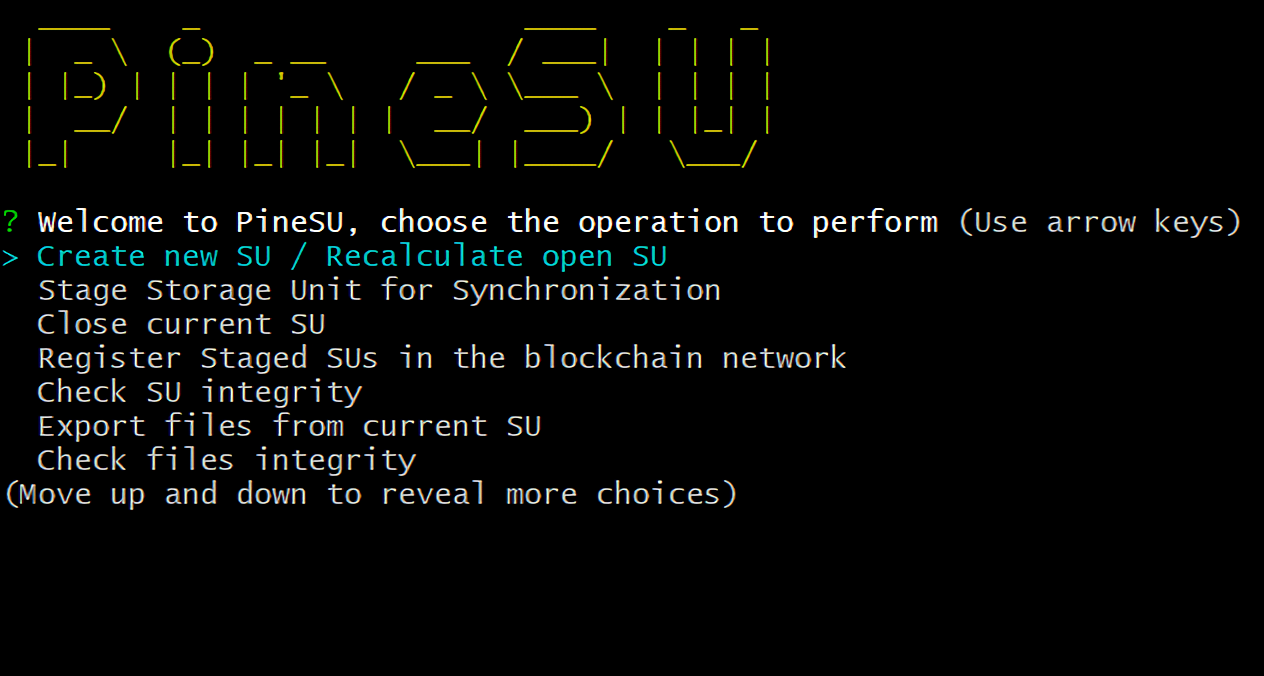
\includegraphics[width=\textwidth]{figures/ops/1.png}
	\end{figure}
\end{frame}

\begin{frame}[fragile]
	\frametitle{Creazione di una Storage Unit (2 di 2)}
	\begin{figure}
		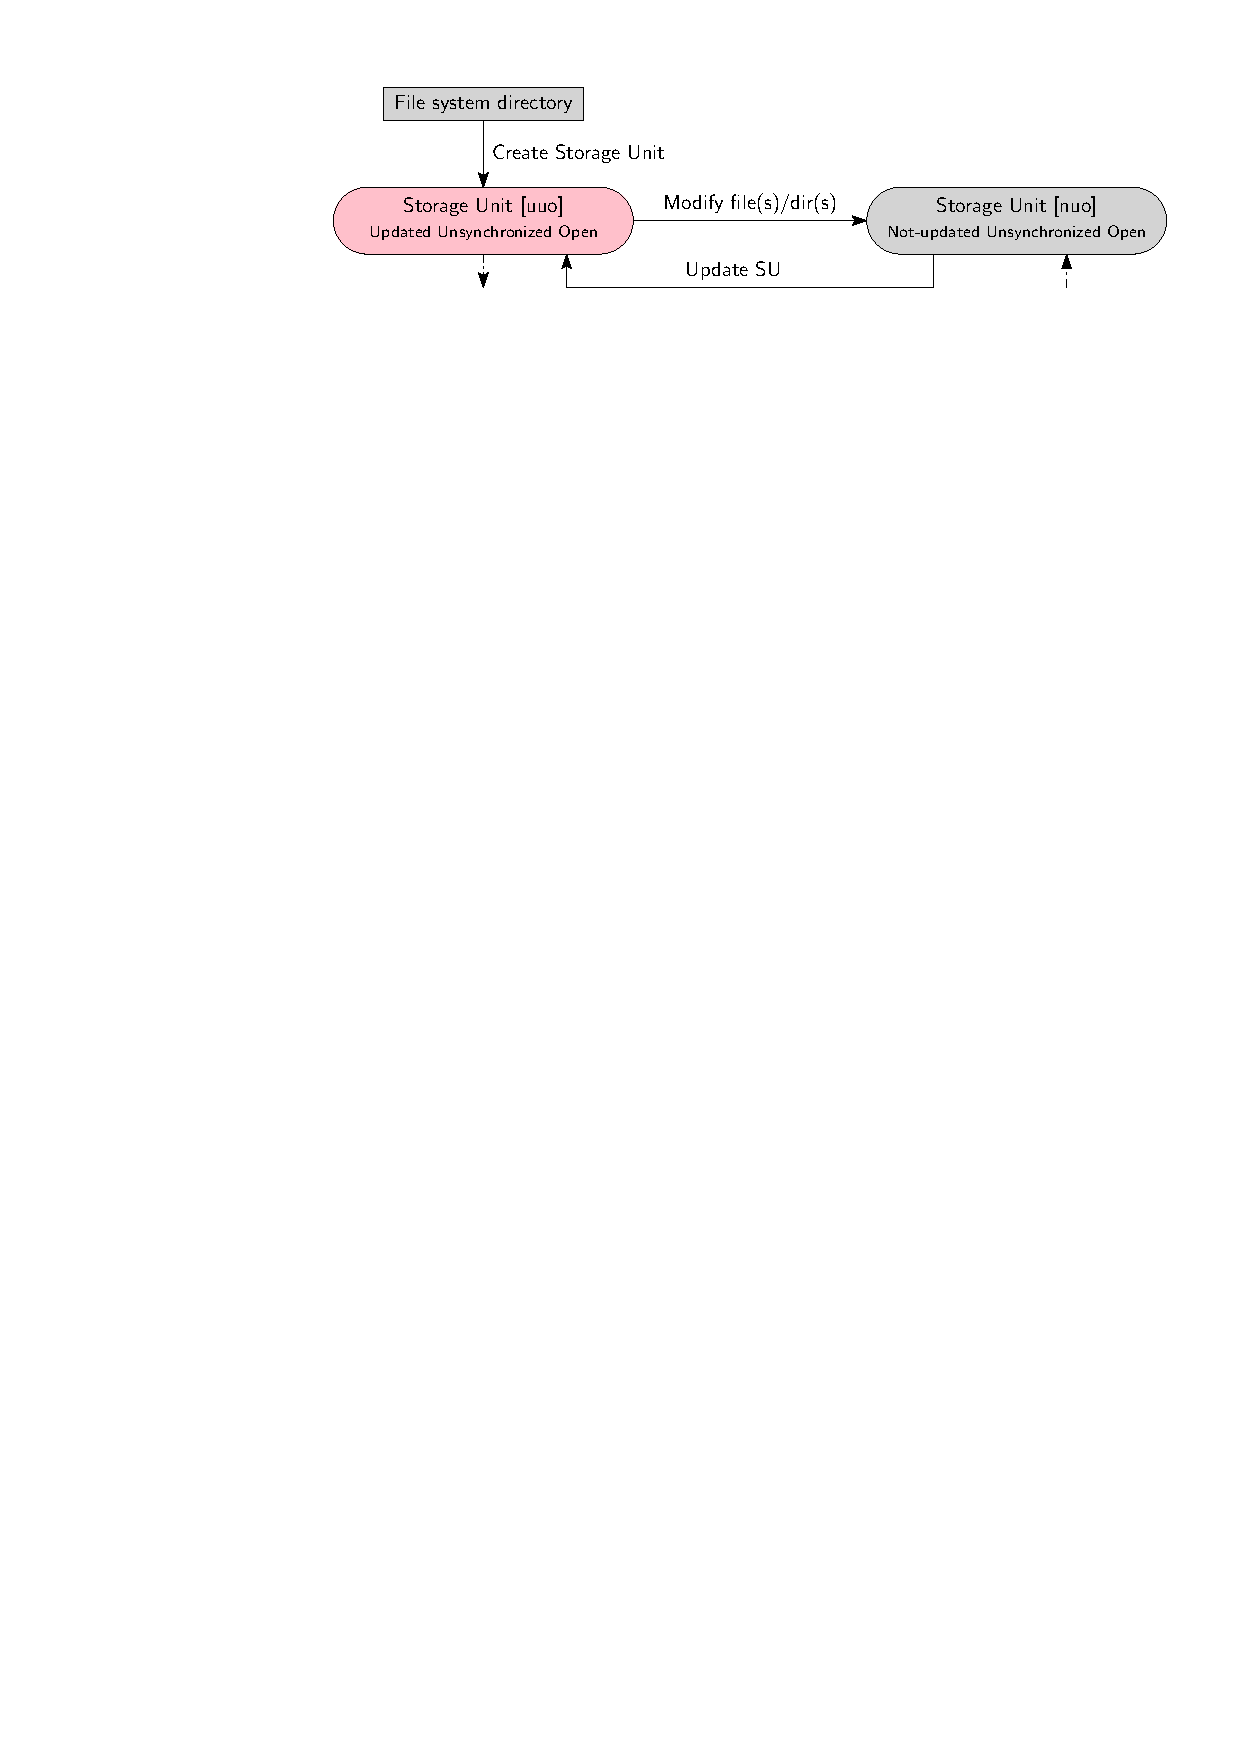
\includegraphics[width=0.8\textwidth]{figures/uuo.pdf}
	\end{figure}
	\begin{columns}
		\column{0.4\textwidth}
		\begin{figure}
			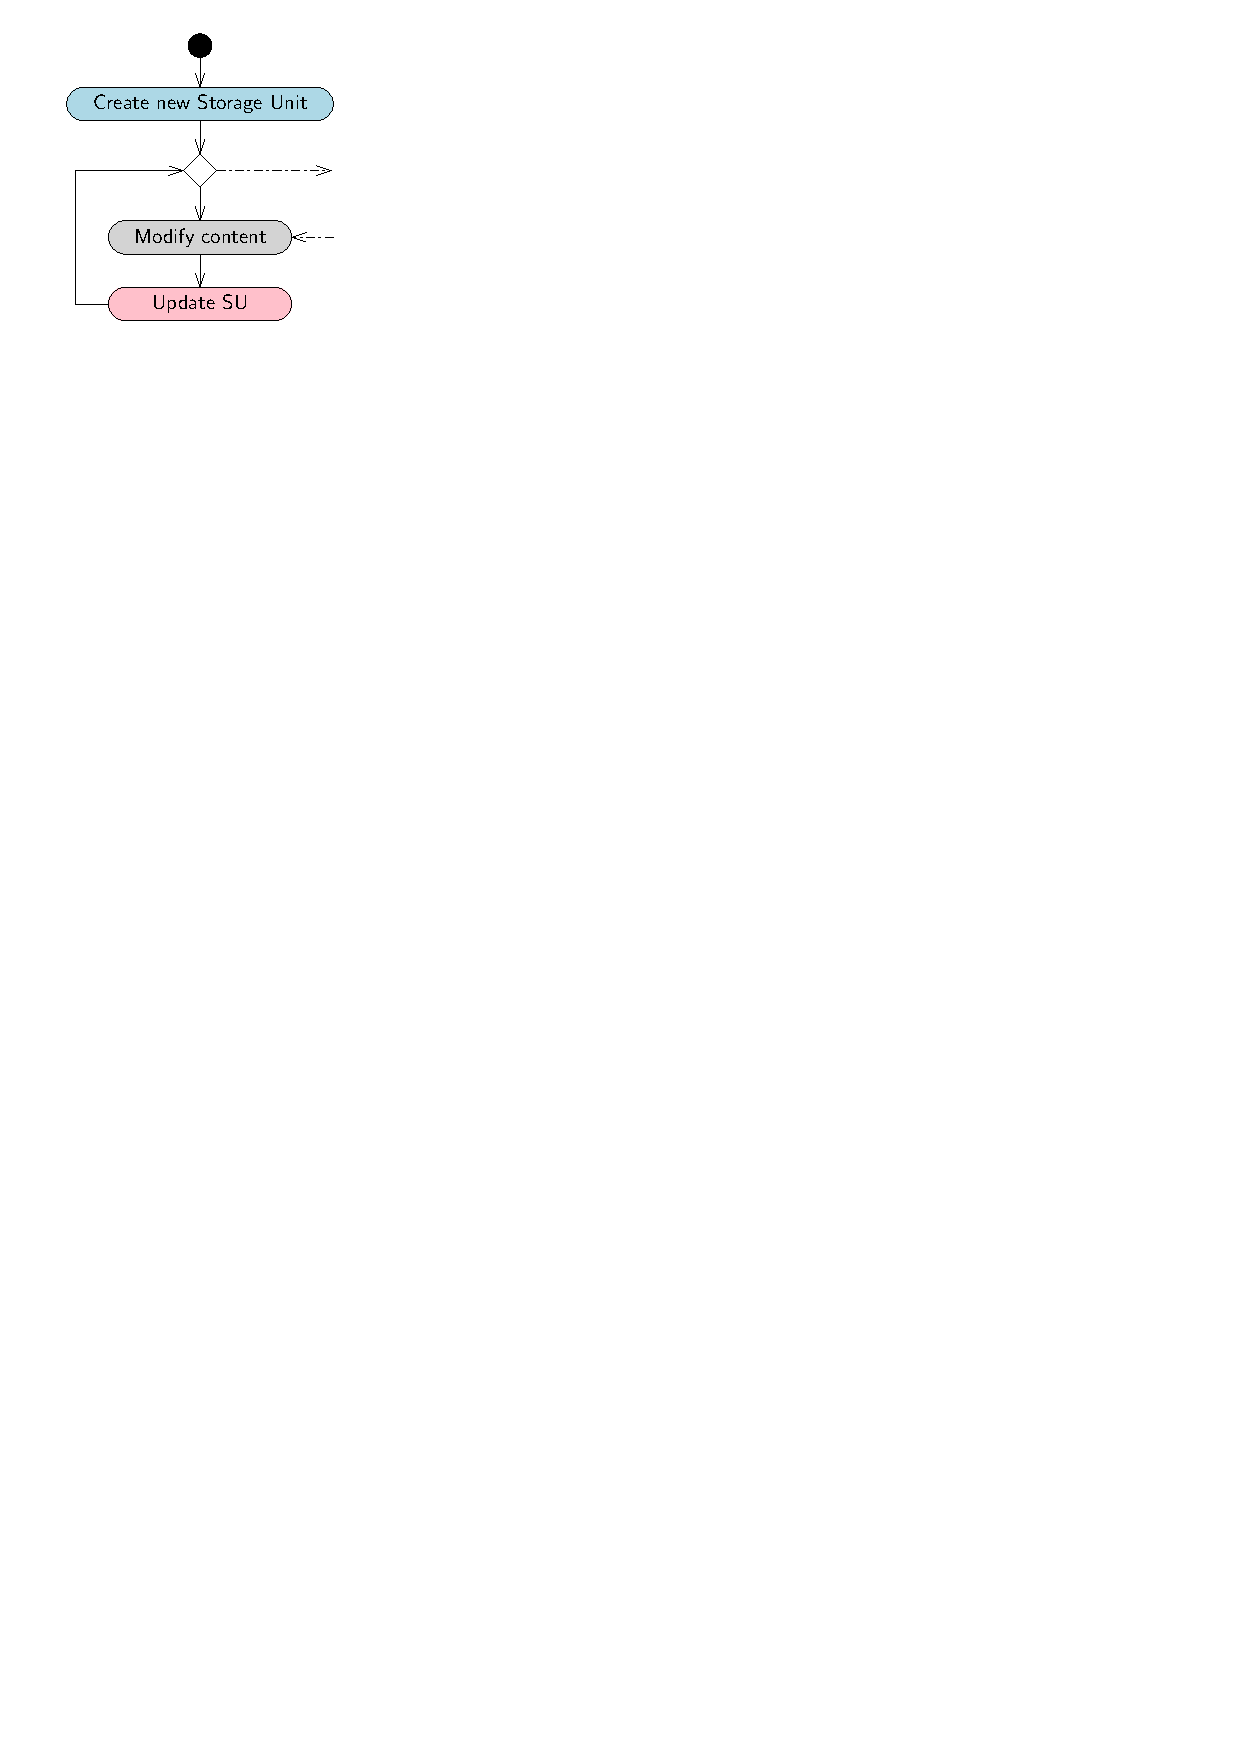
\includegraphics[width=0.8\textwidth]{figures/create.pdf}
			\bigskip
		\end{figure}
		\column{0.6\textwidth}
		\begin{lstlisting}[language=JavaScript, numbers=none]
		var merkleroot =
		 gitLogic.calculateTree(filelist);
		await inquirer.askSUDetails(
			files.getCurrentDirectoryBase(),
			remote).then((details) => {
			details.owner = w1
			details.hash = merkleroot
			details.filelist = filelist
			details.closed = false
			files.saveJSON(details);
		});
		\end{lstlisting}
	\end{columns}
\end{frame}

\begin{frame}
	\frametitle{Registrazione di uno Storage Group (1 di 2)}
	\begin{figure}
		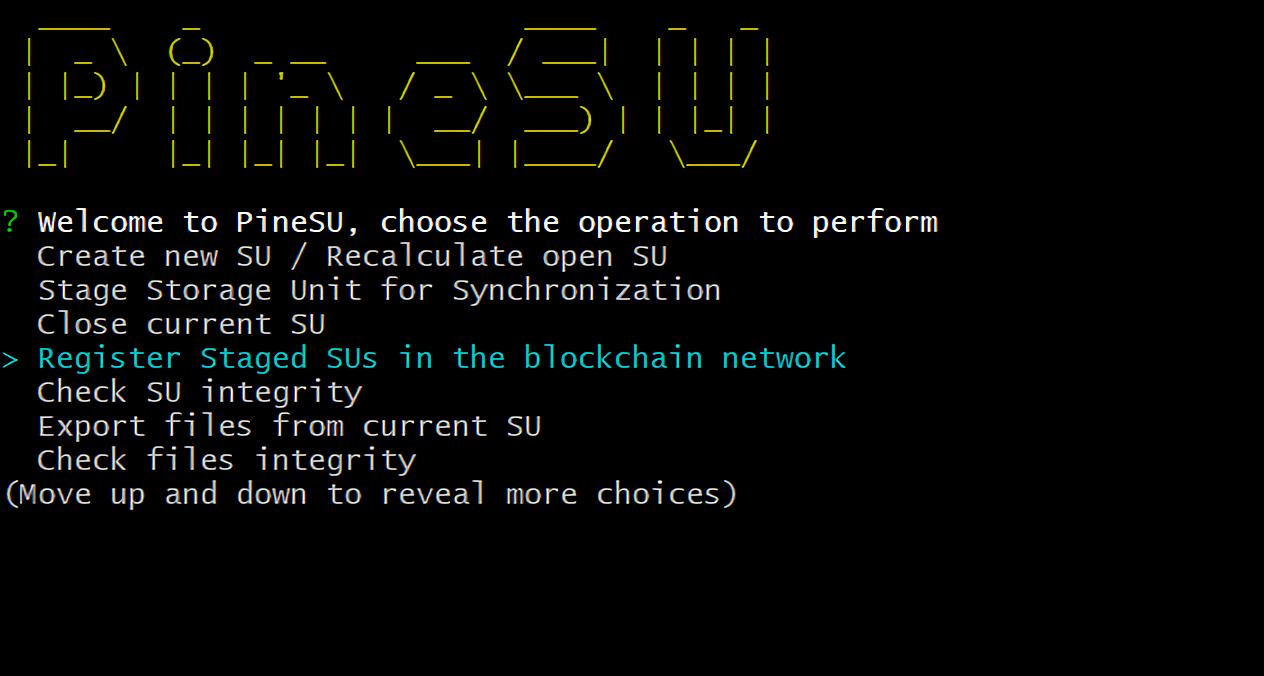
\includegraphics[width=\textwidth]{figures/ops/4.png}
	\end{figure}
\end{frame}

\begin{frame}[fragile]
	\frametitle{Registrazione di uno Storage Group (2 di 2)}
	\begin{figure}
		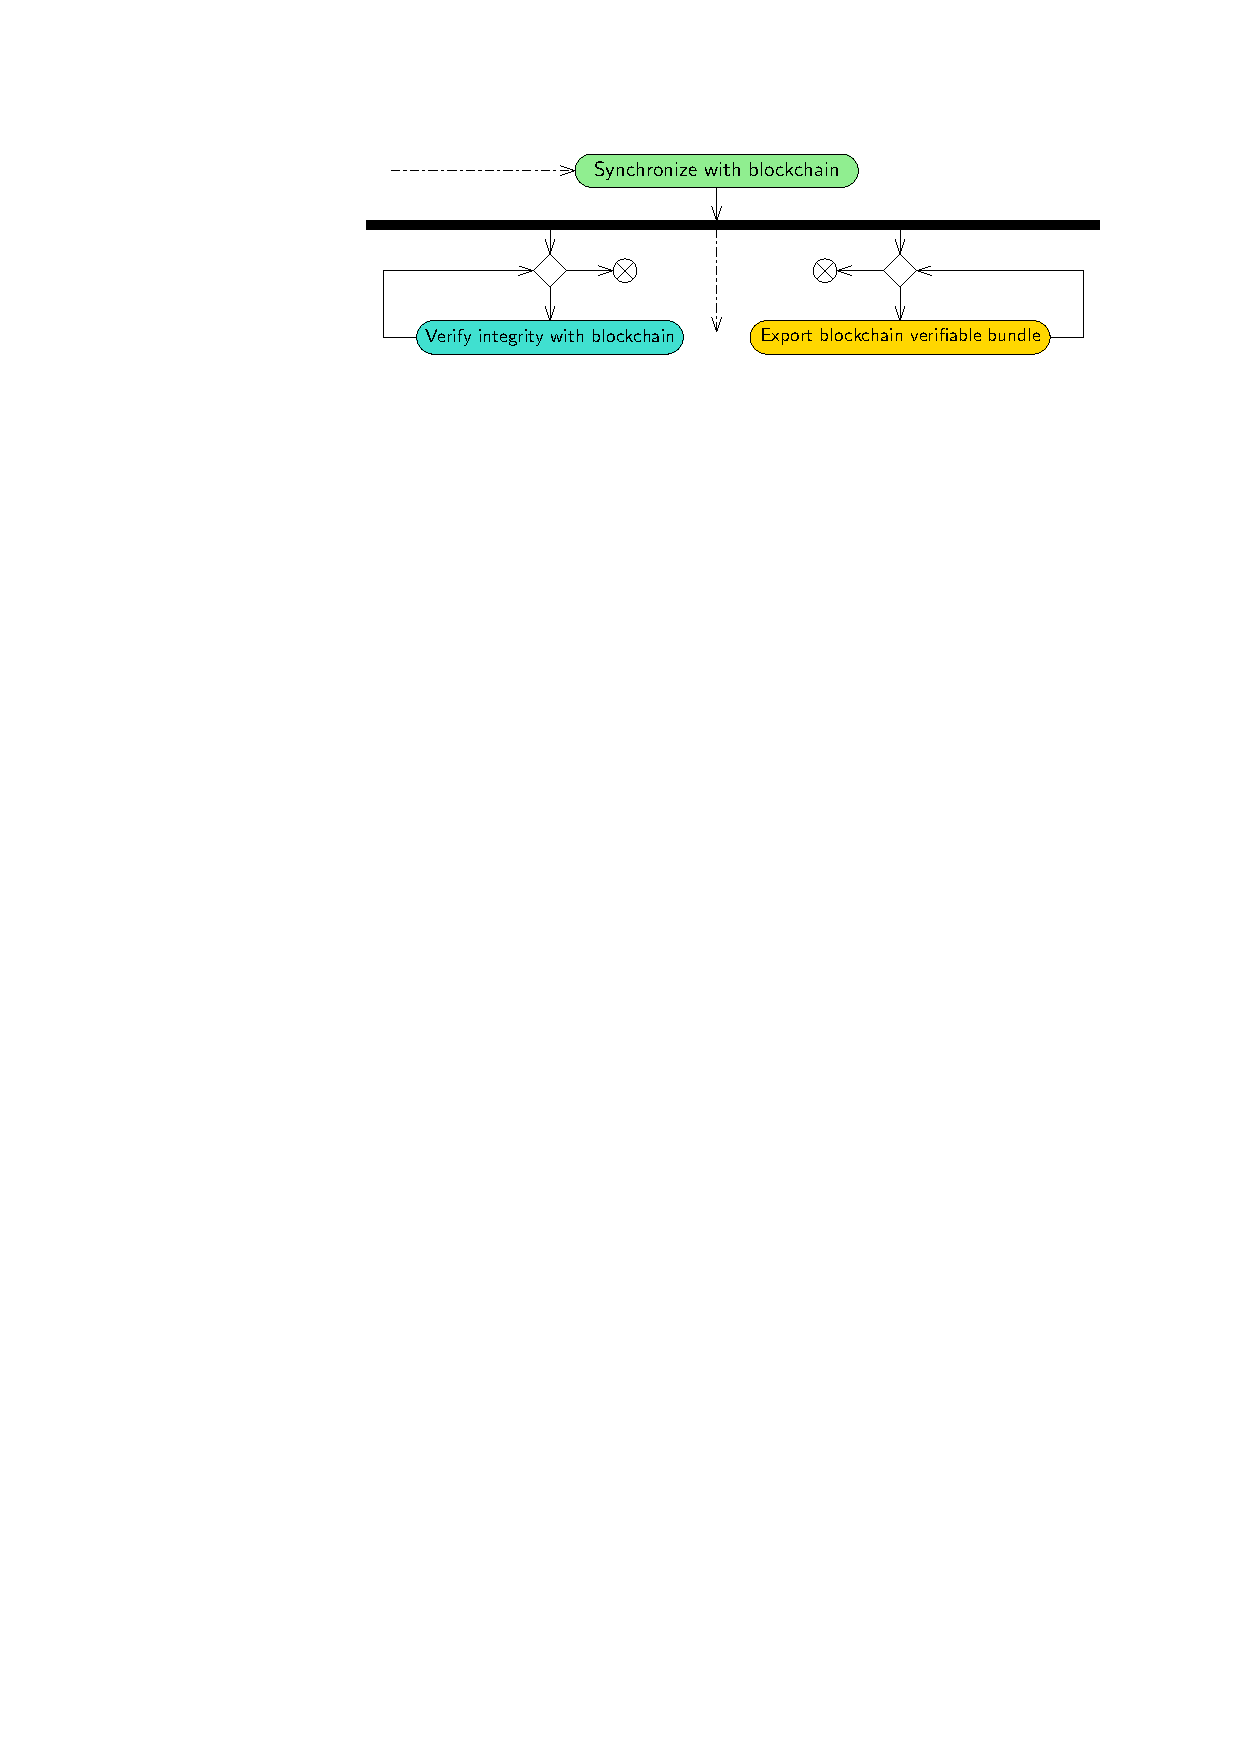
\includegraphics[width=0.8\textwidth]{figures/sync.pdf}
	\end{figure}
	\begin{columns}
		\column{0.6\textwidth}
		\begin{lstlisting}[language=JavaScript, numbers=none]
			var [doc, openRoot, closedRoot] =
				files.createSGTrees(sg);
			ethLogic.
			 addToTree(openRoot, mc, false);
			ethLogic.
			 addToTree(closedRoot, mc, true);
			var [oHash, cHash, transHash] =
			 await ethLogic.registerMC(mc);
			for(var el of document){
				el.transHash = transHash;
				files.createReg(el);
			}
		\end{lstlisting}
		\column{0.4\textwidth}
		\begin{figure}
			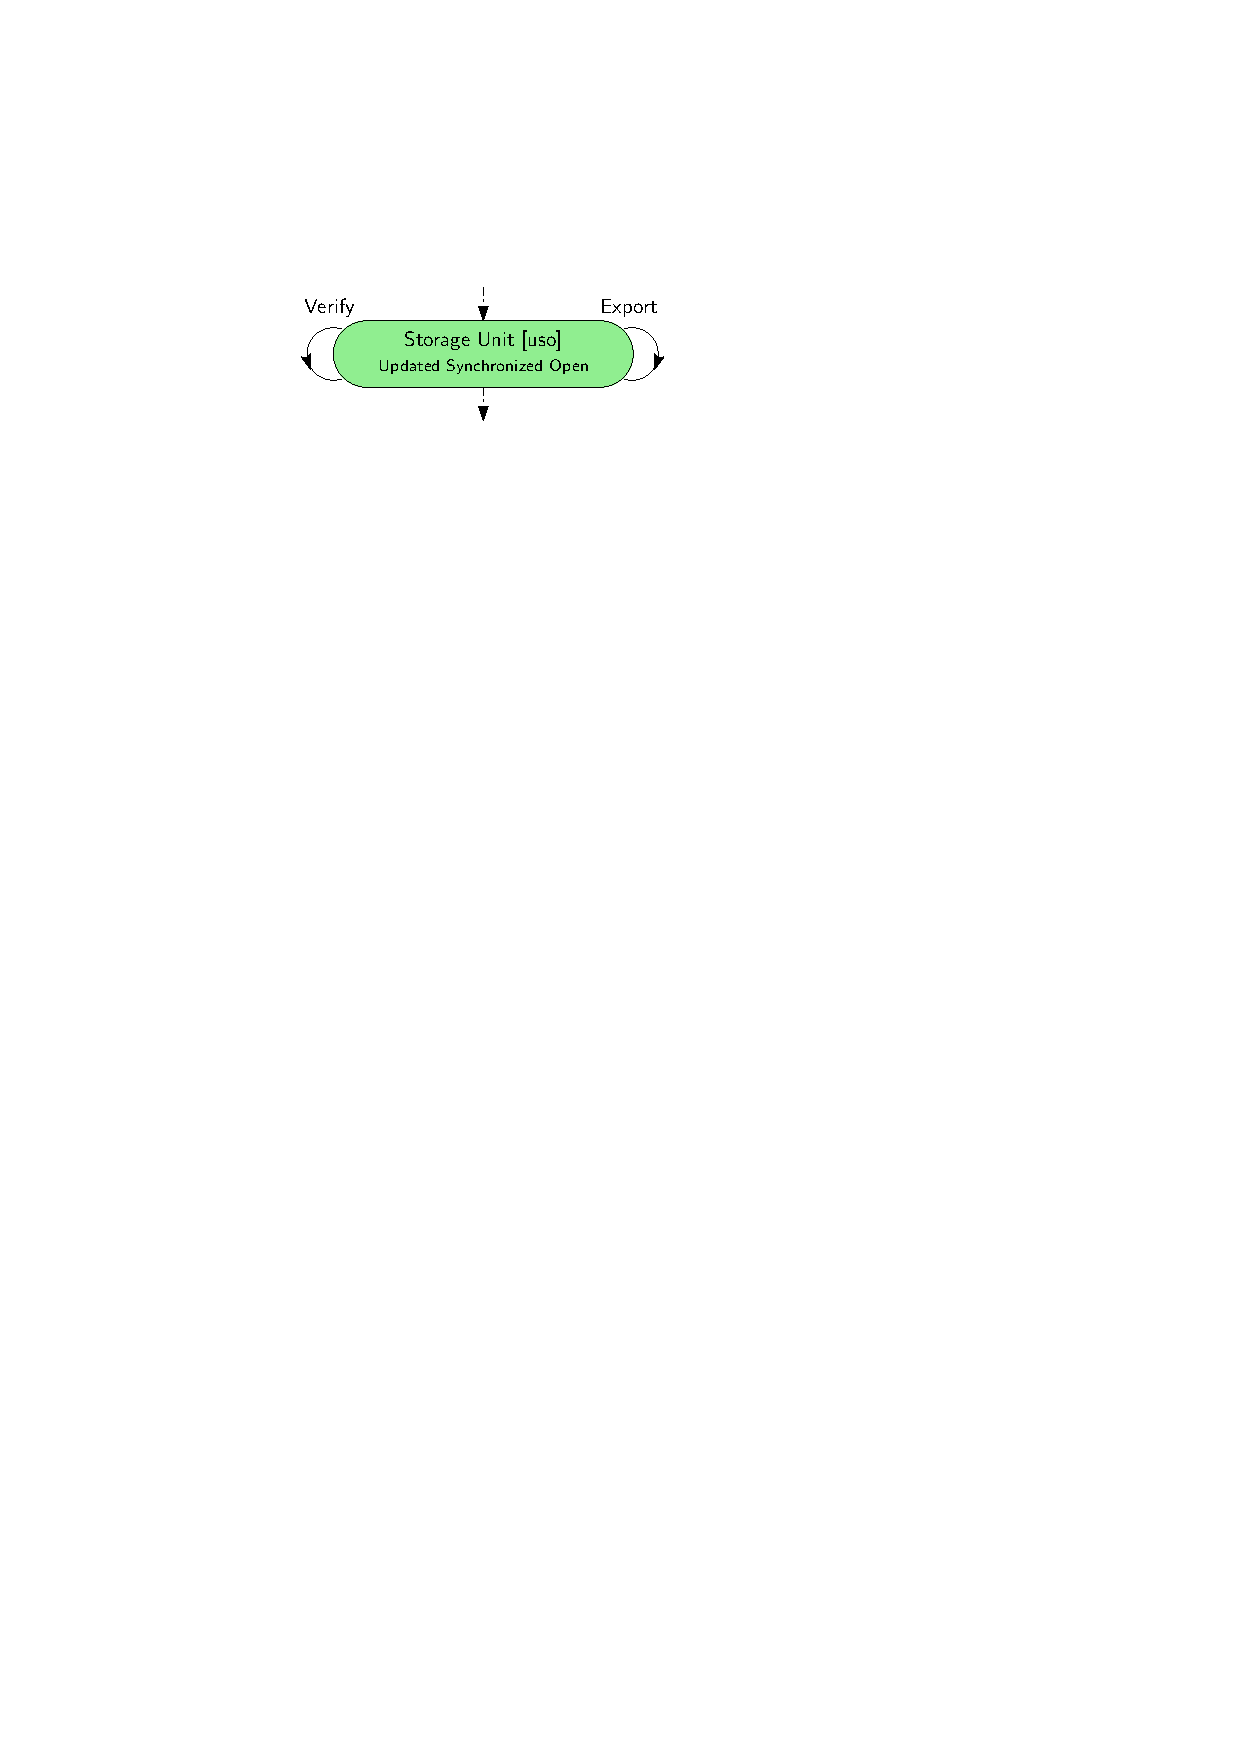
\includegraphics[width=\textwidth]{figures/uso.pdf}
			\bigskip
		\end{figure}
	\end{columns}
	\vspace{-0.6cm}
	\hspace{-0.4cm}
	{\scriptsize La \textbf{registrazione} equivale qui alla \textbf{sincronizzazione}.}
	% registrazione = sincronizzazione
\end{frame}

\begin{frame}[fragile]
	\frametitle{Visualizzazione post-registrazione}
	\begin{columns}
		\column{0.5\textwidth}
		\begin{figure}
			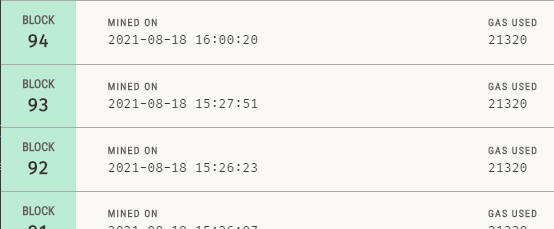
\includegraphics[width=\textwidth]{figures/blocks.png}
		\end{figure}
		\column{0.5\textwidth}
		\begin{figure}
			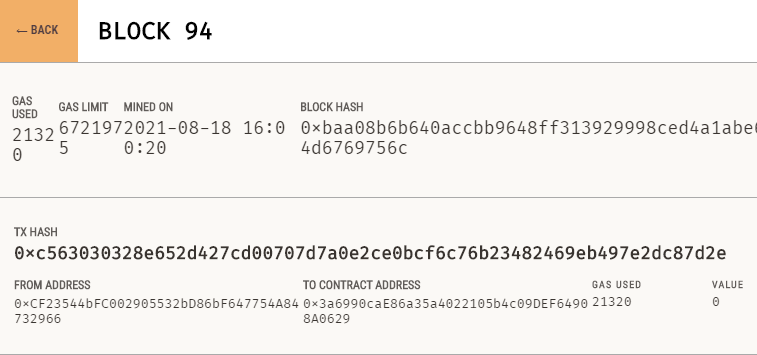
\includegraphics[width=\textwidth]{figures/block.png}
		\end{figure}
	\end{columns}
	\begin{columns}
		\column{0.5\textwidth}
		\begin{figure}
			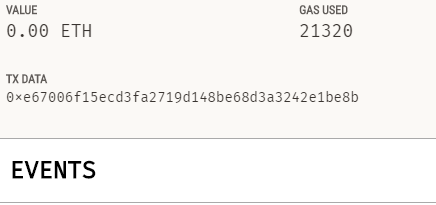
\includegraphics[width=\textwidth]{figures/block2.png}
		\end{figure}
		\bigskip
		\column{0.5\textwidth}
		\begin{lstlisting}[language=JavaScript, numbers=none]
			|\color{blue}"path"|:
				"D:/sample",
			|\color{blue}"root"|:
				"e67006f15ecd3[...]e6
				8d3a3242e1be8b",
			|\color{blue}"transHash"|:
				"0xc563030328e[...]69eb497e2dc87d2e"
		\end{lstlisting}
	\end{columns}
\end{frame}

\begin{frame}
	\frametitle{Chiusura di una Storage Unit (1 di 2)}
	\begin{figure}
		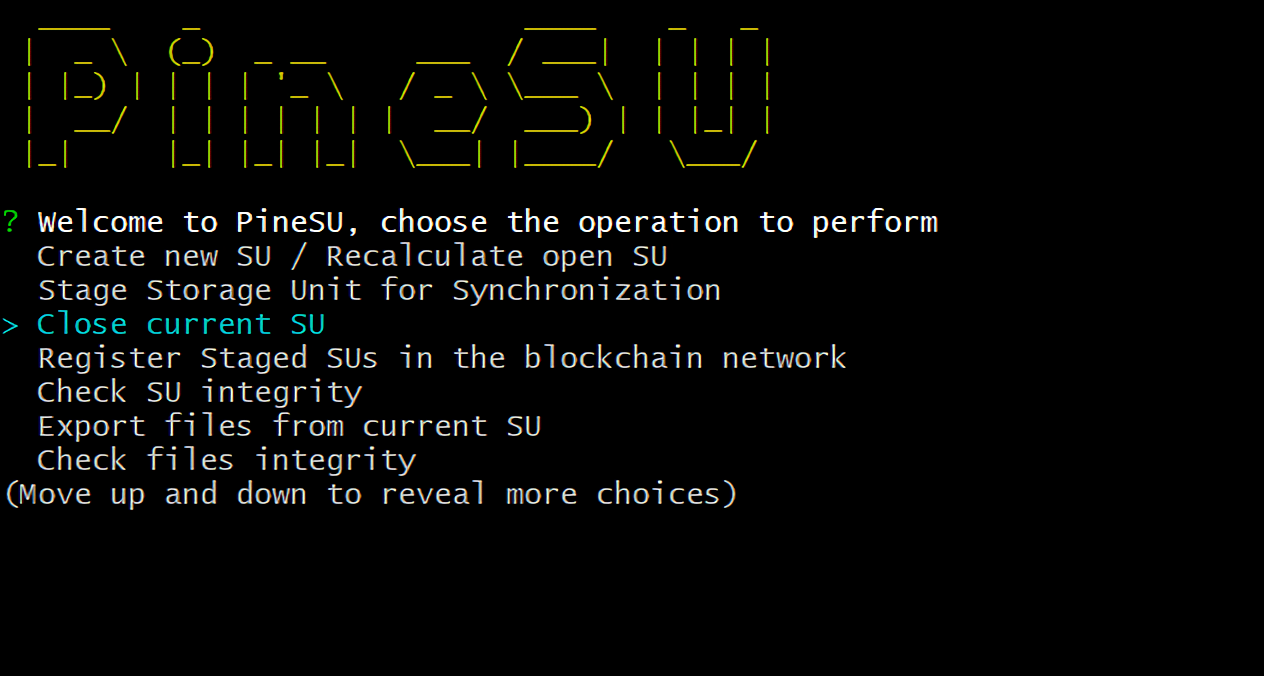
\includegraphics[width=\textwidth]{figures/ops/3.png}
	\end{figure}
\end{frame}

\begin{frame}[fragile]
	\frametitle{Chiusura di una Storage Unit (2 di 2)}
	\begin{figure}
		\includegraphics[width=0.8\textwidth]{figures/closed.pdf}
	\end{figure}
	\begin{columns}
		\column{0.4\textwidth}
		\begin{figure}
			\includegraphics[width=\textwidth]{figures/usc.pdf}
			\bigskip
		\end{figure}
		\column{0.6\textwidth}
		\begin{lstlisting}[language=JavaScript, numbers=none]
			if(fs.existsSync(".pinesu.json")){
				var data = 
				 fs.readFileSync(".pinesu.json")
				var myObj = JSON.parse(data);
				myObj.closed = true;
				fs.writeFileSync(".pinesu.json",
					JSON.stringify(myObj));
				return myObj;
			}
		\end{lstlisting}
	\end{columns}
\end{frame}

\begin{frame}
	\frametitle{Esportazione di bundle di Storage Unit (1 di 2)}
	\begin{figure}
		\includegraphics[width=\textwidth]{figures/ops/6.png}
	\end{figure}
\end{frame}

\begin{frame}[fragile]
	\frametitle{Esportazione di bundle di Storage Unit (2 di 2)}
	\begin{figure}
		\includegraphics[width=0.6\textwidth]{figures/export.pdf}
	\end{figure}
	\begin{lstlisting}[language=JavaScript, numbers=none]
	var zip = new AdmZip()
	var fl = JSON.stringify(json)
	zip.addFile(".pifiles.json", Buffer.alloc(fl.length, fl))
	for(var el of list){
		zip.addLocalFile(path)
	}
	zip.writeZip("/../pinesuExport.zip")
	\end{lstlisting}
\end{frame}

\begin{frame}
	\frametitle{Controllo d'integrità su una Storage Unit (1 di 2)}
	\begin{figure}
		\includegraphics[width=\textwidth]{figures/ops/5.png}
	\end{figure}
\end{frame}

\begin{frame}[fragile]
	\frametitle{Controllo d'integrità su una Storage Unit (2 di 2)}
	\begin{figure}
		\includegraphics[width=0.6\textwidth]{figures/verify.pdf}
	\end{figure}
	\begin{lstlisting}[language=JavaScript, numbers=none]
	async verifyHash(transHash, hash){
		const res =
			await this.web3.eth.getTransaction(transHash)
		if(res.input == "0x"+hash){
			return true;
		} else {
			return false;
		}
	}
	\end{lstlisting}
\end{frame}

\section{Tecnologie utilizzate}

\begin{frame}
	\frametitle{Tecnologie utilizzate}
	\begin{columns}
		\column{0.3\textwidth}
		\begin{itemize}
			\item \textbf{Node.js}
			\item \textbf{JSON}
			\item \textbf{web3.js}
			\item \textbf{Simple Git}
			\item \textbf{Inquirer.js}
			\item \textbf{Chalk}
			\item \textbf{ADM-ZIP}
		\end{itemize}
		\column{0.35\textwidth}
		\centering
		\begin{figure}
			\includegraphics[width=0.7\textwidth]{figures/node.png}
		\end{figure}
		\begin{figure}
			\includegraphics[width=0.7\textwidth]{figures/web3.jpg}
		\end{figure} 
		\bigskip
		\column{0.35\textwidth}
		\centering
		\bigskip\bigskip\bigskip
		\begin{figure}
			\includegraphics[width=0.5\textwidth]{figures/inquirer.png}
		\end{figure}
		\bigskip\bigskip
		\begin{figure}
			\includegraphics[width=0.7\textwidth]{figures/chalk.png}
		\end{figure} 
	\end{columns}
\end{frame}

% git e blockchain hanno potenzialità
% pinesu è un punto di partenza
% tuttavia potrebbe essere semplificato migliorato e velocizzato
% nella blockchain salvando solo
% gli hash riduciamo al minimo l'esposizione di dati
\section{Conclusioni e Sviluppi futuri}
\begin{frame}
	\frametitle{Conclusioni}
	% ridire obiettivo al passato.
	\textbf{PineSU}, sfruttando saggiamente l'interazione tra \textbf{Git} e \textbf{blockchain},
	riesce ad effettuare efficientemente salvataggi e verifiche d'integrità di file.\\
	Inoltre, assicura \textbf{facilità} d'utilizzo e \textbf{minima esposizione} dei propri dati.\\
	L'implementazione attuale è però solo un \textbf{punto di partenza} che, dato il potenziale,
	con ulteriori sviluppi che lo \textbf{migliorino} e \textbf{velocizzino}, potrebbe diventare un'importante risorsa.
\end{frame}

% non fare telecronista
% le persone devono capire che la tesi ha ottime motivaz.
% che ho fatto un sistema intelligente
% dimostro che c'è una modellazione logica
% c'è stata un'implementazione

\begin{frame}
	\frametitle{Sviluppi futuri}
	\begin{enumerate}
		\item Migliorare gestione degli \textbf{accumulatori crittografici} per le \textbf{singole SU}.
		\item Impedire tramite \textbf{Smart Contract} la modifica di SU chiuse.
		\item Aggiungere \textbf{connettori} per \textbf{ulteriori blockchain}.
		\item Creare \textbf{portale web} con \textbf{server Git} per la gestione remota delle SU.
	\end{enumerate}
\end{frame}


\begin{frame}

\end{frame}

%\section{Fonti}
%\begin{frame}
%	\frametitle{Fonti}
%	\begin{itemize}
%		\item \href{https://ethereum.org/it/developers/}{Strumenti Ethereum per sviluppatori} 
%  		\item \href{https://www.trufflesuite.com/tutorial}{Tutorial Truffle DAPPs - Pet Shop}
%  		\item \href{https://www.sitepoint.com/javascript-command-line-interface-cli-node-js/}{Build a JavaScript CLI with Node.js}
%  		\item \href{https://developer.mozilla.org/en-US/docs/Learn/JavaScript/Asynchronous/Async_await}{Tutorial di Mozilla su async / await}
%  		\item Immagini reperite dai siti ufficiali degli strumenti eccetto per alcune scaricate da queste pagine web:
%			\begin{itemize}
%				\item \href{https://www.poeticoding.com/hashing-a-file-in-elixir/}{Funzioni di Hashing}
%				\item \href{https://www.romatoday.it/attualita/concorso-rai-fiera-roma-norme-covid-19.html}{Concorso pubblico}
%				\item \href{https://www.criptovalute24.com/ethereum-migliora-la-sua-blockchain-rialzo-del-5-4/}{Ethereum Blockchain}
%				\item \href{https://blog.netsons.com/git-software-guida-facile/}{Git repository}
%				\item \href{https://amerlin.keantex.com/programmazione-asincrona-con-async-await-parte-2/}{async / await}
%				\item \href{https://transparency.dev/verifiable-data-structures/}{Merkle Tree}
%			\end{itemize}
%			\item \href{https://waifu2x.booru.pics/Home/index}{Strumento di upscaling delle immagini} 
%	\end{itemize}
%\end{frame}

\begin{frame}
	\frametitle{Gli strumenti attuali per la condivisione di documenti}
	\medskip
	\begin{columns}
		\column{0.65\textwidth}
		Uno strumento digitale solitamente segue uno di questi due paradigmi:
		\textbf{centralizzato} e \textbf{distribuito}. \\
		Nel primo un'entità centrale si occupa dell'\textbf{immagazzinamento} e della \textbf{verifica} dei dati
		degli utenti.\\ Ciò ha diversi \textbf{svantaggi}:
		\begin{itemize}
			\item Potenziali attacchi all'entità
			\item Possibile uso malevolo dei nostri dati
			\item Alti costi d'intermediazione
		\end{itemize}
		\column{0.35\textwidth}
		\begin{figure}
			\includegraphics[width=0.90\textwidth]{cent.png}
			% https://icon-icons.com/it/icona/centralizzato-rete-dati-blockchain-tecnologia/95906
		\end{figure}
	\end{columns}
\end{frame}

\begin{frame}
	\frametitle{Strumenti distribuiti}
		Usando invece \textbf{un'architettura distribuita}, sia per la \textbf{gestione dei file},
		sia per la \textbf{verifica delle informazioni}, saremo in grado costruire uno strumento
		che può affidarsi alla parola di una \textbf{moltitudine di entità}, rendendo molto
		più complicati e rilevabili attacchi e manomissioni.
	\medskip
	\begin{figure}
		\includegraphics[width=0.70\textwidth]{dece.jpg}
		% https://docs.microsoft.com/it-it/archive/msdn-magazine/2018/july/blockchain-decentralized-applications-with-azure-blockchain-as-a-service
	\end{figure}
\end{frame}

\begin{frame}
	\frametitle{Accumulatori crittografici}
	\begin{columns}
		\column{0.38\textwidth}
		\begin{figure}
			\includegraphics[width=0.9\textwidth]{figures/mt1.pdf}
		\end{figure}
		\column{0.62\textwidth}
		Strumenti che \textbf{comprimono molte informazioni}
		in una \textbf{costante} di dimensione fissa.
		
		Un esempio ne sono i \textbf{Merkle Tree}, alberi binari
		in cui ogni foglia corrisponde all'hash di un elemento.
		Risalendo ogni nodo interno calcolerà il proprio hash
		con gli hash dei nodi figli, l'hash della root
		sarà \textbf{univoco} a quelle foglie in quell'ordine.
	\end{columns}
\end{frame}

\begin{frame}
	\frametitle{Gli accumulatori di PineSU}
	\begin{columns}
		\column{0.5\textwidth}
		\begin{itemize}%[<+->]
			\item \emph{SU Merkle Tree}: Le sue \textbf{foglie} sono gli \textbf{hash dei file e directory} della SU.\\La sua \textbf{root} è l'\textbf{hash della SU} stessa. 
			\item \emph{Storage Group (\textbf{SG})}: Le sue \textbf{foglie} sono le \textbf{SU da registrare} su blockchain nella prossima transazione.
			\item \emph{Merkle Calendar (\textbf{MC})}.
		\end{itemize}
		\column{0.5\textwidth}
		\centering
		\begin{figure}
			\includegraphics[width=\textwidth]{figures/sg1.pdf}
			\caption{Uno Storage Group}
		\end{figure} 
	\end{columns}
\end{frame}

\begin{frame}
	\frametitle{Node.js}
	\begin{columns}
		\column{0.7\textwidth}
		\textbf{Node.js} è un \textbf{ambiente di run-time},
		che permette di eseguire codice \textbf{Javascript}.
		\smallskip \\
		Esso ha come obiettivi chiave l'\textbf{efficienza} 
		e la \textbf{scalabilità}, può infatti eseguire
		velocemente codice Javascript sia \textbf{server-side}
		che \textbf{client-side}.\\
		\smallskip
		Parte fondamentale di Node sono
		i suoi numerosi \textbf{moduli}: librerie e framework
		realizzati dalla comunità e installabili con facilità
		tramite il package manager \textbf{npm}
		\column{0.3\textwidth}
		\centering
		\begin{figure}
			\includegraphics[width=\textwidth]{figures/node.png}
		\end{figure} 
	\end{columns}
\end{frame}

\begin{frame}
	\frametitle{Moduli dei connettori}
	\begin{columns}
		\column{0.7\textwidth}
		\textbf{web3.js} è un \textbf{modulo npm} che permette di
		interagire con \textbf{nodi Ethereum} locali e remoti.\\
		\smallskip
		\emph{PineSU EC} lo utilizza per effettuare le \textbf{transazioni} con i
		suoi wallet e per comunicare con lo \textbf{Smart Contract}. \\
		\column{0.3\textwidth}
		\centering
		\begin{figure}
			\includegraphics[width=\textwidth]{figures/web3.jpg}
		\end{figure} 
	\end{columns}
	\medskip
	\begin{columns}
		\column{0.3\textwidth}
		\centering
		\begin{figure}
			\includegraphics[width=0.75\textwidth]{figures/gitfw.png}
		\end{figure} 
		\column{0.7\textwidth}
		\textbf{Simple Git} è un \textbf{modulo npm} che permette di
		comunicare con il \textbf{client Git} locale. \\
		\smallskip
		Usato in \emph{PineSU GC}, esso permette l'esecuzione di
		comandi in maniera \textbf{asincrona}. \\
	\end{columns}
\end{frame}

\begin{frame}
	\frametitle{Altri moduli}
	\begin{columns}
		\column{0.3\textwidth}
		\centering
		\begin{figure}
			\includegraphics[width=0.75\textwidth]{figures/inquirer.png}
		\end{figure} 
		\column{0.7\textwidth}
		\textbf{Inquirer.js} è un \textbf{modulo npm} che facilita
		la creazione di \textbf{interfacce utente} tramite menù testuali. \\
		\smallskip
		In \emph{PineSU CLI} viene usato per \textbf{interagire}
		con l'utente ponendogli \textbf{domande} dalla risposta chiusa o aperta. \\
	\end{columns}
	\medskip
	\begin{columns}
		\column{0.72\textwidth}
		\textbf{ADM-ZIP} è un \textbf{modulo npm} che consente di
		creare \textbf{cartelle compresse} in formato ZIP.\\
		\smallskip
		\emph{PineSU BEL} lo utilizza per \textbf{esportare sottoinsiemi} di
		SU mantenendo la \textbf{struttura gerarchica} originale. \\
		\column{0.28\textwidth}
		\centering
		\begin{figure}
			\includegraphics[width=0.88\textwidth]{figures/zip.png}
		\end{figure} 
	\end{columns}
\end{frame}

\end{document}